\documentclass{article}
\usepackage{todonotes}
\usepackage{graphicx} % Required for inserting images
\usepackage{tabularx}
\usepackage{hyperref}
\usepackage{authblk}
\usepackage{natbib}
\usepackage[margin=1in]{geometry} %This command sets the margins of the document to 1 inch on all sides
\renewcommand{\baselinestretch}{1.5} %This command sets the line spacing of the document to 1.5 times the default value.
\newcommand*{\para}{\par\vspace{\baselineskip}\noindent} %command is defined to insert a paragraph break followed by a vertical space
\usepackage{float}
\usepackage{appendix}
\usepackage{multicol}
\usepackage{adjustbox}
\setlength\parindent{0pt}
\usepackage{caption}
\usepackage{subcaption}
\usepackage{adjustbox}
\usepackage{multirow}
\usepackage{mathtools} %This command loads the mathtools package, which provides various tools for typesetting mathematical expressions, such as special symbols, functions, and constructs.
\usepackage{amsmath,amssymb,amsthm,enumerate,tikz,arydshln,ragged2e,wasysym} %This command loads several additional packages that provide additional math-related features, such as symbols, functions, and constructs for typesetting math expressions, as well as tools for drawing figures and diagrams.
\usepackage{pdfpages}
\usepackage{verbatim}

\usepackage{tikz}
% \usetikzlibrary{arrows}
\usetikzlibrary{trees}

\newtheorem{example}{Example} %environment is defined to format examples
\newtheorem{lemma}{Lemma}
\newtheorem{proposition}{Proposition}
\newtheorem{theorem}{Theorem}
\newtheorem{conjecture}{Conjecture}

\newcommand{\euler}{e}

\newcommand{\argmax}{\operatornamewithlimits{argmax}} %command is defined to represent the mathematical argmax operator.

% \usepackage{subfigure}

\bibliographystyle{abbrvnat}

\title{Master Thesis}
\author{Tom McGrath}
\date{\today}

\begin{document}

\begin{titlepage}

	\centering
	
	\includegraphics[width=0.5\textwidth]{UM}\par\vspace{3cm}

	{\huge\bfseries Competitive Secretary Problem \par}
	
	{\scshape\Large Master Thesis \par}
	
	\vspace{2cm}
	
	{\Large\itshape	Tom McGrath  }

        i6223829
	
	\vfill
	
	supervised by\par
	Marc \textsc{Schröder}

	\vfill

	{\large \today\par}
	
\end{titlepage}

\begin{abstract}
This thesis explores a competitive variant of the classic secretary problem, introducing a strategic candidate who has the ability to manipulate their interview position. We delve into the optimal strategies for both the employer and the strategic candidate, considering the employer's objective to hire the best candidate and the strategic candidate's goal to be hired. The research employs a game-theoretic approach to model the strategic interactions between the employer and the candidate. It provides analytical expressions for the optimal strategies and utilities under different conditions. The thesis also investigates the effects of different weighting systems on the likelihood of a candidate being strategic, revealing interesting dynamics in the competitive setting. It suggests potential directions for future research, including empirical testing of the model and exploration of other strategic behaviors in the secretary problem. The findings of this thesis contribute to our understanding of strategic decision-making in hiring processes and provide insights that could be valuable for both employers and job applicants. The research also has potential implications for other areas where similar decision-making dynamics occur, such as online auctions and dating.
\end{abstract} 
\newpage
\tableofcontents
\thispagestyle{empty}
\listoffigures
\listoftables
\newpage
\pagenumbering{arabic}

\section{Introduction}

The secretary problem is one of the most well known examples of an optimal stopping problem. It goes by a myriad of other names too, being known as the marriage problem, the sultan's dowry problem, the fussy suitor problem, the googol game, and the best choice problem. The multitude of names for this problem indicates its extensive study over the years, with \cite{dynkin1963optimum} determining the optimal stopping rule for this problem. The problem which was first stated in the February 1960 issue of \textit{Scientific American}, and has become a sub-field of study within mathematics-probability-optimisation \cite{ferguson1989solved} and the comprehensive review paper authored by \cite{freeman1983secretary} illuminates the remarkable scope and magnitude that the field has acquired. Furthermore, it is evident that the field has persistently witnessed exponential expansion since the publication of that seminal paper.
\\[2ex]
The premise of the secretary problem involves selecting the best option from a sequence of choices (secretaries, potential spouses, etc.) based on a single observation for each choice. The objective is to maximize the probability of choosing the best option, and the choices must be made sequentially. There are $n$ applicants who are all ranked from $1$ to $n$, with $1$ being the best. The applicants are interviewed one by one in random order and immediately after each interview, an irrevocable hiring decision is made. The decision is made knowing only how that candidate compares to all other candidates seen up till that point. Moreover, an applicant that has been rejected cannot later be hired. The optimal strategy in this setting is to wait till $e^{-1}$, where $e$ is the base of the natural logarithm, of the candidates have been interviewed, rejecting them all and choosing the first applicant that is better than all the ones seen so far. This leads to a probability of $e^{-1}$ of selecting the best one. This is the optimal choice in the limit as the number of applicants tends towards infinity.
\\[2ex]
The exact origins of the problem are shrouded in ambiguity, while it can be understood that the secretary problem is one that has been encountered since the beginning of man, the academic origins of the problem can be traced back to the mid-20th century. The problem's early history is somewhat obscure, with multiple researchers contributing to its development. This historical note aims to shed light on the various accounts surrounding the problem's inception. \cite{gilbert196620} mentions that in 1955, A. Gleason posed the secretary problem, but the exact origins of his formulation remain unclear. Gleason likely encountered the puzzle through informal discussions or encounters with other mathematicians, as there is no definitive record of its source. One notable figure associated with the secretary problem is \cite{gardner1960mathematical}, who attributed the problem to J.H. Fox and L.G. Marnie in 1958. However, the circumstances under which Fox and Marnie introduced the problem are not well-documented, leaving room for speculation on their contribution. After this various special cases of the problem were solved which further drove the development of this problem, until there was the famous $e^{-1}$ result that we know of today. After this point many variants were created and studied.
\\[2ex]
In the competitive secretary problem, the focus of my thesis, an element of competition is added. This fundamentally changes the nature of the problem, transforming it from an optimisation problem of optimal stopping theory to one of game theory. Now, instead of a single decision maker, there are multiple competing parties. These could be multiple employers vying for the best applicant, or a competition between an employer and a strategic candidate. The introduction of these competitive elements makes the problem more realistic and applicable to real-world scenarios, secretary problems have been gaining a lot of relevance in modern times regarding online auctions. In the traditional secretary problem, there is a single decision maker who is trying to maximize their chance of choosing the best option. However, when a competitive element is added, there are now multiple decision makers who are all trying to maximize their own chances of success. This changes the problem from an optimization problem to a game theory problem, as each decision maker must now consider not only their own choices, but also the potential choices of their competitors.
Building on this base problem, researchers have explored a plethora of extensions. These include variations in the objective function, the information available to the decision maker, and the number of choices the decision maker can make, among others. One extension involves varying the objective function, which changes the criteria for what constitutes the 'best' choice. Another extension involves changing the information available to the decision maker. Yet another extension involves changing the number of choices the decision maker can make, such as allowing them to hire multiple applicants or to reconsider rejected applicants. Some key works in this area include those by \cite{ajtai2001improved}, \cite{freeman1983secretary},and \cite{gilbert2006recognizing}. The relevance of this research extends beyond academia, offering key insights into the dynamics of the labour market. In many decentralised labour markets, candidates are offered positions at very early stages in the hiring process. It has been argued that this early timing of offers is due to competition among employers for the best applicant. Indeed, \cite{immorlica2006secretary} show that as the number of competing employers grows, the timing of offers becomes earlier, confirming this hypothesis.
% This research is relevant for employers and prospective employees, it can give key insights into some of the dynamics of the labour market. In many decentralised labour markets, candidates are offered positions at very early stages in the hiring process and it has been argued that this is due to competition among employers for the best applicant. \cite{immorlica2006secretary} show that this is indeed the case and that as the number of competing employers grows, the timing of offers becomes earlier.
\\[2ex]
Within this broader field, my thesis focuses on a specific variant of the competitive secretary problem, where the employer and a strategic candidate are competing. The strategic candidate who is chosen from the set of applicants with uniform probability can choose where in the interview process to position themselves and the employer can choose how many people they will search through before seriously considering applicants. This variant has been studied before in work by \cite{buchbinder2014secretary}. They solve it using position independent algorithms which they find via linear programming, they show that there exists a position independent algorithm that selects the best candidate with probability $\approx 0.29$. In this thesis, we take a different approach and instead of using linear programming we will directly define each agents utility function and find the optimal strategies players can employ.
\\[2ex]
The outline of this thesis is as follows, first we will perform a literature review of the competitive secretary problem and the different variants that have been studied over the years. We will then introduce the problem by means of a leading example. The model will then be introduced and it will be solved via backwards deduction, starting in the full information setting and the choice of the strategic applicant then moving to the choice of the employer. The employer is pitted against the second ranked applicant who is the toughest competition for the employer.  We then move to the incomplete information setting where the employer is not aware of which candidate is strategic. The asymptotic nature of the employers actions are studied. The assumption of uniform weights of a candidate being strategic is dropped and more weighting functions are explored. Then a comparison to the classic secretary problem is made, followed by two extensions where the applicant is made unaware of their rank and multiple strategic candidates are introduced. This is followed by a discussion on the possible extensions and future research. Finally a conclusion is made.

\subsection{Literature Review}

In \cite{immorlica2011dueling}, the authors  study classic algorithmic search and optimisation problems from the perspective of competition. All the games are two player zero sum games, where the objective is simply to beat the opponent rather than try maximise their score or minimise cost. Two main questions are studied by the authors. 1. Will players use the classic optimisation solution in a dueling setting? An algorithm is called $\beta$-beatable (over probability distribution $p$) if there exists a response which achieves a payoff $\beta$ against that algorithm (over probability distribution $p$). For the secretary problem, referred to as the hiring duel in the two player context, the authors find an upper bound of 0.82 and lower bound of 0.51. The lower bound follows from the fact that the symmetric equilibrium strategy $\pi$, revealed below beats the classical algorithm with probability bounded above $0.5$ when the classical algorithm hires early (i.e., before round $\frac{n}{2}$), and the upper bound follows from the fact that the classical algorithm guarantees a probability of $\frac{1}{e}$ of hiring the best candidate, in which case no algorithm can beat it.
\\[2ex]
The second question the authors address is 2. What strategies do players play at the equilibrium? An algorithm is said to efficiently solve the duel if it takes as input a representation of the game, probability distribution p and outputs an action $x \in X$ distributed according to some minmax optimal (i.e Nash) strategy. In the hiring duel the symmetric equilibrium $\pi $ is as follows, if the opponent has already hired, then hire anyone who  beats his employee; otherwise hire as soon as the current candidate has at least a $50\%$ chance of being the best of the remaining candidates.
\\[2ex]
In work done by \cite{karlin2015competitive}, they investigate how the competition between multiple ranked employers competing to hire the best candidate from a common pool of candidates. They derive subgame-perfect nash equilibrium strategies and analyse the impact the competition has on the quality of the hires as a function of the rank if the employer. There are $k$ totally order employers and n totally ordered applicants. The ranking of the employers is to break ties and the applicant will choose the employer with the highest rank in the case that multiple offers are made.
\\[2ex]
There are two objectives considered for the employers, the first is when each employer is trying to maximise the probability of hiring the very best applicant. Dynamic programming is used to find a subgame-perfect Nash equilibrium for this game. A subgame is the game that remains after $m$ applicants have arrived. Consider, for example, the case where $k = 2$, in which exactly two employers, say I and II, are competing for the best candidate. The strategy of employer I, the top-ranked employer, is simple: he just runs the standard secretary algorithm, since offers made by employer II would always be rejected in favor of offers from employer I. Employer II, on the other hand, must take employer I’s strategy into account. It turns out that the best (subgame-perfect) response for employer II in the limit is to wait until an $e^{-3/2}$ fraction of the candidates have been interviewed, and then make offers to any candidate better than the best seen so far, until employer II successfully hires someone. (Employer II’s first offer might be to the same person employer I makes an offer to, so II might end up making 2 offers.) Also, just as the top employer has probability $e^{-1}$ of success (the same as the fraction of candidates he interviews before considering any offer), the probability that II successfully hires the best applicant is in fact $e^{-3/2}$. More generally, the lower the rank of the employer, the earlier they will start making offers and, of course, the lower their probability of success.
\\[2ex]
The second objective studied is when, for each $j$, the j-th ranked employer seeks to hire any one of the top $j$ applicants. A subgame-perfect Nash Equilibrium is also found for this objective. The structure of such an equilibrium is as follows, Consider, say the j-the ranked employer. Then there is a set of numbers $\alpha_1 > \alpha_2 > ... > \alpha_j $ between 0 and 1 such that employer j will attempt to make an offer to the i-th best applicant so far or better after an $\alpha_i $ fraction of applicants have been seen. However, these thresholds vary over time, depending on whether higher ranked employers have already hired someone or not. After higher-ranked employers have hired, the thresholds increase, i.e., an employer’s standards go up as applicants are snapped up by higher ranked employers and competition from these employers has ceased.
\\[2ex]
In \cite{immorlica2006secretary}, a different variant of the two employer game is presented, which provides a new derivation of the resulting symmetric two player mixed-Nash equilibrium, and then proceed to study $k$ player extension of this game. One of the properties of any strategy for the employer game is its threshold time, which is defined as the largest fraction $\tau$ such that the strategy is guaranteed not to make
an offer to any of the first $\tau$ candidates, no matter what the player observes nor what the other players do. They show that in any pure Nash equilibrium of the k-employer game, at least one of the players has a threshold time $\tau \leq \frac{2}{k}$. Next a more realistic version of the game, in which the players are allowed to use adaptive strategies, which base their decisions on the opponent’s past actions as well as the public information revealed thus far. This defines a multi-player stochastic game. They describe the unique subgame perfect mixed Nash equilibrium of this game as the solution of a dynamic program. Using properties of the dynamic program, they prove that the timing of the first offer converges to zero as the number of players tends to infinity. More precisely, every player’s threshold time is at most $\frac{1}{k}$.
\\[2ex]
The paper "Secretary Problems via Linear Programming" by \cite{buchbinder2014secretary} introduces a novel approach to the classical secretary problem and its variants using linear programming (LP) techniques. The authors propose a linear program formulation that establishes a correspondence between algorithms for the secretary problem and feasible solutions to the LP. This formulation offers several advantages, including the ability to compute the optimal algorithm by solving a linear program, proving upper bounds on algorithm performance by finding feasible solutions to the dual program, and exploring problem variants through the addition of constraints or manipulation of the objective function. The authors demonstrate the applicability of their approach by exploring the J-choice, K-best secretary problem, where the algorithm aims to select the best candidates among n arrivals by choosing up to J candidates from the top K ranked candidates. They provide a linear program that characterizes all algorithms for this problem, extending the framework to capture a broad range of algorithmic strategies.
\\[2ex]
In addition, the paper investigates position independent algorithms for the secretary problem, where the probability of selecting a candidate is equal for each position. The authors show the existence of position independent algorithms that select the best candidate with a probability of $1-\frac{1}{\sqrt{2}} $ and prove their optimality. They address the limitations of the optimal position independent algorithm by introducing regret-free and must-hire algorithms that ensure the selection of candidates better than all previous ones and always hire a candidate, respectively. The linear programming technique is employed to derive and prove the optimality of these algorithms.
\\[2ex]
The significance of this paper lies in its development of a comprehensive LP-based framework for the secretary problem and its variants. By formulating the problem as a linear program, the authors provide a powerful tool for computing optimal algorithms, establishing performance bounds, and exploring problem variations. The paper contributes to the existing literature by extending the applicability of LP techniques to encompass the J-choice, K-best secretary problem and position independent algorithms. These findings not only enhance our understanding of the secretary problem but also have implications for related domains, such as online auctions. Overall, the paper presents a systematic and rigorous approach that advances the study of the secretary problem and provides valuable insights for algorithm design in decision-making scenarios.
\\[2ex]
In the paper "The Postdoc Variant of the Secretary Problem" by \cite{vanderbei1983postdoc}, a variant of the classic secretary problem is explored. The author introduces a scenario where the goal is not to select the best candidate, but rather the second-best one. This is motivated by the idea that the best candidate is likely to accept an offer from a more prestigious institution (e.g., Harvard). The author refers to this as the "postdoc problem". Vanderbei models this as a sequential decision problem and provides an explicit solution for both the optimal strategy and the associated optimal success probability. The optimal strategy involves rejecting the first half of the applicants and then accepting the first applicant who is second-best so far. The probability of success using this strategy is approximately 1/4, suggesting that it is harder to select the second-best from a pool of applicants than it is to select the best. The author also explores the problem of selecting the m-th best candidate out of n, providing a general formula for the probability of ending up with the m-th best choice given that this person is currently known to be the j-th best out of the first k interviewed. However, explicit solutions are only provided for the cases where m equals 1, 2, n, and n-1. The problem of picking the median candidate from an odd-sized pool is identified as particularly interesting, but left for future work.

\subsection{Leading Example}

To illustrate the concepts and strategies discussed in this thesis, consider the following example. Suppose a tech company is hiring for a software engineer position. The employer has decided to interview a total of 10 applicants. Each applicant has a unique skill level, represented by a natural number. The employer's goal is to hire the applicant with the highest skill level. The applicants, on the other hand, aim to maximize their chances of being hired. The applicants are ordered into a list where being in the first position refers to being of the best rank and the target of the employer.
\\[2ex]
In this Stackelberg game, the employer moves first by deciding the number of applicants ($\ell$) to search through before making a decision. The strategic applicant, knowing the employer's strategy, will then choose their position in the interview process. The employer will reject the first $\ell$ candidates and select the first candidate that is better than the best candidate that appeared in the first $\ell$ interviews.

\begin{example}
Consider a set of 10 applicants, each with a unique ID and skill level. Clearly the best candidate is that with ID 7, this applicant is so much better that it is clear that the employers goal is to hire applicant 7 and getting the second best, candidate 9, is still very far off from optimal. The table on the left shows the ID and skill level of each applicant. The table on the right shows the same applicants, but ordered by skill level and assigned a rank $k$.

\begin{table}[H]
\begin{minipage}{0.45\textwidth}
\centering
\label{tab:applicants}
\begin{tabular}{|c|c|}
\hline
\textbf{ID} & \textbf{Skill level} \\ \hline
1 & 10 \\ \hline
2 & 6\\ \hline
3 & 44 \\ \hline
4 & 30 \\ \hline
5 & 86 \\ \hline
6 & 42 \\ \hline
7 & 60408 \\ \hline
8 & 89 \\ \hline
9 & 105 \\ \hline
10 & 97 \\ \hline
\end{tabular}
\caption{Applicants}
\end{minipage}\hfill
\begin{minipage}{0.45\textwidth}
\centering
\label{tab:applicants_ranked}
\begin{tabular}{|c|c|}
\hline
\textbf{ID} & \textbf{$K$} \\ \hline
7 & 1 \\ \hline
9 & 2\\ \hline
10 & 3 \\ \hline
8 & 4 \\ \hline
5 & 5 \\ \hline
3 & 6 \\ \hline
6 & 7 \\ \hline
4 & 8 \\ \hline
1 & 9 \\ \hline
2 & 10 \\ \hline
\end{tabular}
\caption{Applicants Ranked}
\end{minipage}
\end{table}

In the classic secretary problem the probability of picking the best one is given by the formula $\frac{\ell}{n}\sum_{i = \ell + 1}^{n}\frac{1}{i-1}$. This formula calculates the probability that the employer will select the best applicant, given that they reject the first $\ell$ applicants. The optimal $\ell$ is $\frac{n}{e}$, so in this example, the optimal $\ell$ is 4. This leads to a probability of picking the best of $39.9 \% $.
\end{example}

\section{The Model}

\subsection{Model Introduction}

The competitive secretary problem variant that is the focus of this thesis can be represented by a Stackelberg leadership model, in which there is a leader, the \emph{employer} and follower, the \emph{applicant} (also known as the \emph{candidate}). A competitive secretary problem (CSP) is triple $(N,k,e)$. The applicant $k$ is in a set $N$ of applicants which is nonempty, finite and ordered. Each applicant $k$ has a rank $k$. Where $k\in \{1, \ldots, n \}$ and $ k=1$ refers to being of the best rank. The employer (e) has the objective to hire the best candidate, that is the applicant of rank $k=1$. Thus, the best strategy she can deploy is one that maximises the probability of picking the best. We restrict the employer to search and exploit strategies, similar to those in the classic secretary problem. The employer before interviewing the candidates must decide on a number $\ell$, this is the number of candidates she will reject regardless of their rank, This is the search phase of her decision problem. After which she will hire the next candidate who is the better than the best candidate seen in $\ell$, that is, that candidate will be the best candidate seen so far. Additionally, there is one strategic candidate ($k$) who is of rank $k$ and has the ability to decide where in the interview process he will position himself. As the candidate is the follower he will choose this after the employer has decided on her $\ell$. The goal of the candidate is to be hired and so his best strategy is one that maximises the probability of being picked. The payoff for being picked is 1 and 0 for not being picked, while the payoff for the employer is 1 for selecting the best candidate and 0 otherwise. The candidate chooses a number $\alpha$ which refers to where after $\ell$ he would like to position himself. Let $CSP^N$ denote the domain of all competitive secretary problems with set of players $N$.
\\[2ex]
The employer's strategy space is choosing a $\ell\in\{0,1,\ldots, |N|-1\}$. We restrict the choice to search and exploit strategies. This means that the employer first searches through candidates, rejecting them one by one, and then after an interval of searching, begins exploiting, which in this case means having the possibility to accept an applicant. The space of possible strategies is restricted due to the sequential decision-making aspect of the game. Additionally, as decisions are irrevocable, the employer must commit to the current candidate or continue to search for a better one. Lastly, the employer can only rank the candidate relative to the ones previously interviewed, but there's no way to compare them to ones that have not been interviewed yet. Therefore, the employer's best strategy is to first search through a certain number of candidates to gather information about the quality of the candidate pool (the search phase), and then to start seriously considering candidates for the position (the exploit phase). This strategy maximizes the employer's chances of selecting the best candidate. You can find more about this in the classical literature on the secretary problem. The employer can search through as many people as she would like but must hire someone. So, she cannot search through everyone and will be forced to hire the last person if she has not hired someone else. \\
The strategic candidate's strategy space is choosing an $\alpha \in \{1,\ldots,|N|-l \} $. $\alpha = 1$ refers to the first position after $\ell$ while $|N|-l$ refers to positioning himself at the end. We do not consider the applicant as having the choice to position themselves within $\ell$. Thus a (pure) strategy profile for this game is a vector $((\ell),(\alpha))$.
\\[2ex]
In all formulae going forward, $n$ refers to $|N|$. In Stackelberg games, it is a common assumption that if the follower is indifferent between two or more strategies, they will break the tie in favor of the leader. This assumption is made because the Stackelberg model is a leadership model where the leader moves first and the follower moves after observing the leader's action. The follower, knowing the leader's strategy, can at best respond optimally to the leader's action. If there are multiple optimal responses, the follower is assumed to choose the one that is most favorable to the leader. This assumption simplifies the analysis of the game and ensures that the leader's optimal strategy can be determined without having to consider multiple possible responses from the follower for each of the leader's possible actions. The Stackelberg leadership model is appropriate for this problem because it captures the sequential nature of the decision-making process in the competitive secretary problem. The employer, as the leader, makes the first move by deciding how many candidates to search through. The strategic candidate, as the follower, then decides where to position themselves in the interview process based on the employer's decision. This model accurately reflects the dynamics of the competitive secretary problem and allows us to analyze the strategies of both the employer and the strategic candidate.
\\[2ex]
The utility of candidate $k \in N$ for each $(N,k,e) \in CSP^N $ with $\ell\in\{0,1,\ldots, n-1\}$ and $\alpha \in \{1,\ldots,n-\ell \} $ is given by 
$$ u_{k}(\ell, \alpha) \in [0,1] \text{ for all } k \in \{1, \ldots, n \}.  $$
The utility is the probability of the candidate being picked given the employers choice $\ell$ and the candidates choice $\alpha$. This utility function captures the candidate's goal of maximizing their chances of being hired.
\\[2ex]
% The utility the applicant receives from different choices of $\alpha$ is the probability of being picked given those decisions. The utility of candidate $k\in N$ is defined as follows $$ u : CSP^N \mapsto [0,1]^N $$
% \todo[inline]{You currently define the utility as a function from secretary problems to a vector of probabilities for each of the players. However, an applicant's utility only depends on $\alpha$, so we would only define $u_k(\alpha)$.}
% assigns to each $(N,k,e) \in CSP^N $ the utility $u(N,k,e)\in[0,1]^N$ with $\ell\in\{0,1,\ldots, n-1\}$ and $\alpha \in \{1,\ldots,n-\ell \} $ is given by 
% $$ u_{k}(\ell, \alpha) \in [0,1] \text{ for all } k \in \{1, \ldots, n \}.  $$ 
% \\[2ex]
The utility of the employer for each $(N,k,e) \in CSP^N $ with $\ell\in\{0,1,\ldots, n-1\}$ and $\alpha \in \{1,\ldots,n-\ell \} $ is given by 
$$u_e(\ell, k) \in [0,1] \text{ for all } k \in \{1, \ldots, n \}.  $$ 
The utility the employer receives is the probability of picking the $k=1$ candidate given their choice $\ell$ and the applicants choice of $\alpha$. This utility function captures the employer's goal of hiring the best candidate.
\\[2ex]
These utility functions provide a mathematical representation of the goals of the employer and the strategic candidate. They are influenced by the choices of $\ell$ and $\alpha$, and they guide the strategies of the employer and the strategic candidate in the competitive secretary problem.
\\[2ex]
% The utility the employer receives from different choices of $\ell$ is the probability of selecting the best ranked candidate. The utility of the employer ($e$) picking the best candidate, $k\in N$ and being rank $k =1$ is defined as follows
% $$ u_e : CSP^N \mapsto [0,1] $$ assigns to each $(N,k,e) \in CSP^N $ the probability $u(N,k,e)\in[0,1]$ with $\ell\in\{0,1,\ldots, n-1\}$ and $\alpha \in \{1,\ldots,n-\ell \} $ is given by $$u_e(\ell, k) \in [0,1] \text{ for all } k \in \{1, \ldots, n \}.  $$ 
One of the main concepts relied upon in this thesis is the Nash equilibrium. The Nash equilibrium is when all agents or players can not improve by deviating to another strategy, that is they are all using their best response to each other. The modern concept of Nash equilibrium is defined in terms of mixed strategies, where players choose a probability distribution over possible pure strategies. The concept of a mixed-strategy equilibrium was introduced by \cite{von1944theory}  in their 1944 book 'The Theory of Games and Economic Behavior', but their analysis was restricted to the special case of zero-sum games. They showed that a mixed-strategy Nash equilibrium will exist for any zero-sum game with a finite set of actions. Another concept in game theory are zero-sum games, a zero-sum game is a special type of game where the gains of one player are the same as the losses of another player, so if you were to add all the positive payoffs of players and subtract all the losses of players the resulting sum would be zero, examples of these type of games are chess, go and poker. The contribution of \cite{nash1951non} in his 1951 article "Non-Cooperative Games" that attached his name to the concept was to define a mixed-strategy Nash equilibrium for any game with a finite set of actions and prove that at least one (mixed-strategy) Nash equilibrium must exist in such a game. Since then there have been a number of refinements made, such as subgame perfect equilibrium introduced by \cite{selten1965spieltheoretische}, which looks to see if an equilibrium is still an equilibrium when examining every sub game. The subgame perfect equilibrium (SPE) is the equilibrium concept that will be used in this thesis. A profile $((\ell),(\alpha))$ is a subgame perfect equilibrium when, for each subgame, the restriction of the profile to that subgame is a Nash equilibrium of that subgame. A subgame is a part of the game tree that starts in a singleton information set, and does not have an information set that contains decision nodes both within and outside the subgame. Using these equilibrium concepts implies that that agents are assumed to be rational.
\\[2ex]
Two special cases will now be treated. The first is when $l=0$ is chosen, in this case the employer will not search through any of the candidates and will accept the first candidate they interview.

% In the first variant studied, the employer employs a fixed strategy $\ell$ and knows that $k$ is a strategic candidate. As mentioned in the introduction in the classic secretary problem $ l = \frac{n}{e} $ which is what will be used as the base case. The employer will reject the first $\ell$ candidates and then accept the first candidate which is better than all the ones she has seen thus far, if the best candidate appeared in the first $\ell$ interviews she will then be forced to accept the final candidate interviewed, because she would continue searching for a better candidate than the best in $\ell$, until she arrives at the last candidate and is forced to choose him. The only active player in this first variant is  a strategic candidate who can choose where in the interview order he would like to appear. In all formulae going forward, $n$ refers to $|N|$.
% \\[2ex]
% The probability of candidate $k\in N$ of getting selected is defined as follows
% $$ p : CSP^N \mapsto [0,1]^N $$ assigns to each $(N,k,e) \in CSP^N $ the probability $p(N,k,e)\in[0,1]^N$ with $l\in\{0,1,\ldots, |N|-1\}$ and $\alpha \in \{1,\ldots,|N|-l \} $ is given by $$ p_{k}(l, \alpha) \in [0,1] \text{ for all } k \in \{1, \ldots, n \}.  $$ 

\subsection{Special Case: No Search}

\begin{lemma}\ \label{l=0}
If $\ell=0$, then the best-response of each candidate $k\in N$ is $\alpha=1$. This yields $u_k = 1$ and $u_e=\frac{1}{n}$. \label{lemma:applicant_employer:l=0}
\begin{proof}
Since $l=0$, the employer will always select the first candidate, as any candidate is better than none, as no candidate would report a value of 0, and all candidates are assumed to have a skill value greater than or equal to 0. Thus, the only rational strategy is to choose $\alpha = 1$ as anything else will lead to not being selected. This strategy leads to always being selected for any $k$. Thus, 
$$ u_k(0,\alpha) =
\begin{cases}
    1 & \text{ if } \alpha = 1, \\
    0 & \text{ if } \alpha \neq 1.
\end{cases}
\text{for all } k \in \{1, \ldots, n \}. $$
Given this, we know that any strategic candidate will pick position $\alpha = 1$. If the strategic candidate is known then if $k = 1$ the probability of picking $k=1$ is 1 and if $k\neq1$ the probability of picking $k=1$ is 0. When the strategic candidate $k$ is unknown the probability of the strategic candidate being $k=1$ is $\frac{1}{n}$ as there is an equal chance that any of the candidates are strategic and this is the utility of the employer.
\end{proof}
\end{lemma}

\subsection{Special Case: Best Ranked Applicant is Strategic}

In this case where the strategic candidate is the best ranked candidate that is $k=1$, the game becomes a game of cooperation rather than competition as this is exactly the candidate that the employer would like to hire.

\begin{lemma}\label{lemma:best_strategic}

For $K=1$, in an SPE we have that $u_e=u_1=1$.
\begin{proof}
The $k=1$ candidate will choose $\alpha=1$ as there is nobody better than him, this will lead to him always being selected. This is true for any $\ell$. 
\end{proof}
\end{lemma}

\section{Applicant Perspective - Complete Information}

In this section we will begin the in depth analysis of the game and use backwards deduction to solve the game. The game can be modelled with the following game tree. In the example below there are only two candidates, one of each can be strategic.

\begin{figure}[H]
\label{fig:Game_tree_1}
\centering
\scalebox{1}{
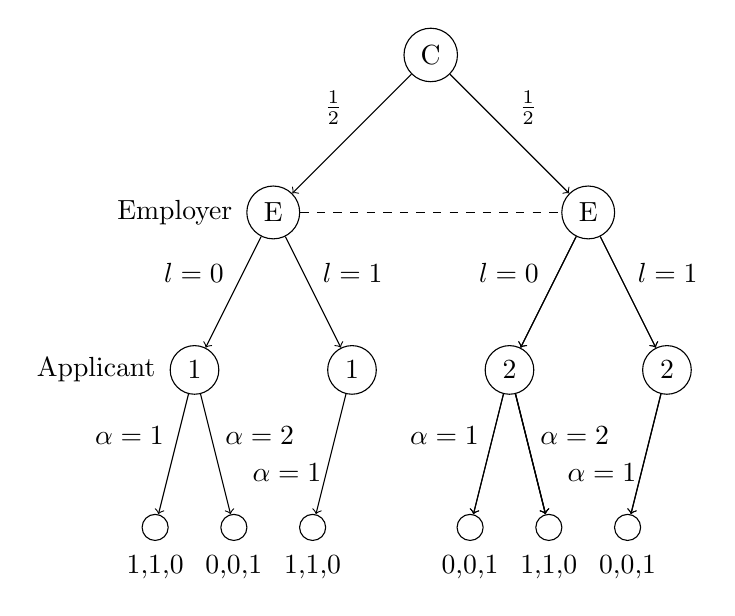
\begin{tikzpicture}
  \node[circle,draw] (1) at (0,0) {C}; % Chance Node
  \node[circle,draw] (2) at (-2,-2) {E}; % k=1 is strategic
  \node[circle,draw] (3) at (2,-2) {E}; % k=2 is strategic
  \node[circle,draw] (4) at (-3,-4) {1};
  \node[circle,draw] (5) at (-1,-4) {1};
  \node[circle,draw] (6) at (-3.5,-6) {};
  \node[circle,draw] (8) at (-2.5,-6) {};
  \node[circle,draw] (9) at (-1.5,-6) {};
  % \node[circle,draw] (11) at (-0.5,-6) {};
  \node[circle,draw] (12) at (1,-4) {2};
  \node[circle,draw] (13) at (3,-4) {2};
  % \node[circle,draw] (14) at (3.5,-6) {I};
  \node[circle,draw] (15) at (2.5,-6) {};
  \node[circle,draw] (16) at (1.5,-6) {};
  \node[circle,draw] (17) at (0.5,-6) {};

  \node at (-3.25,-2) {Employer};
  \node at (-4.25,-4) {Applicant};
  \node at (-3.5,-6.5) {1,1,0};
  \node at (-2.5,-6.5) {0,0,1};
  \node at (-1.5,-6.5) {1,1,0};
  % \node at (-0.5,-6.5) {0,0};
  \node at (0.5,-6.5) {0,0,1};
  \node at (1.5,-6.5) {1,1,0};
  \node at (2.5,-6.5) {0,0,1};
  % \node at (3.5,-6.5) {1,0};
  
  \draw[dashed] (2) to node[above] {} (3);
  \draw[->] (1) to node[above left]{$\frac{1}{2}$} (2);
  \draw[->] (1) to node[above right]{$\frac{1}{2}$} (3);
  \draw[->] (2) to node[above left]{$l = 0$} (4);   
  \draw[->] (2) to node[above right]{$l = 1$} (5); 
  \draw[->] (3) to node[above left]{$l = 0$} (12);   
  \draw[->] (3) to node[above right]{$l = 1$} (13);  
  \draw[->] (4) to node[above left]{$\alpha = 1$} (6);  
  \draw[->] (4) to node[above right]{$\alpha = 2$} (8); 
  \draw[->] (5) to node[below left]{$\alpha = 1$} (9);  
  % \draw[->] (5) to node[below right]{$\alpha = 2$} (11); 
  \draw[->] (12) to node[above left]{$\alpha = 1$} (17);  
  \draw[->] (12) to node[above right]{$\alpha = 2$} (16); 
  \draw[->] (13) to node[below left]{$\alpha = 1$} (15);  
  % \draw[->] (13) to node[below right]{$\alpha = 2$} (14); 

  % Additional lines and arrows
  \draw[->] (3) to (12); % Arrow from node 2 to node 12 (G)
  \draw[->] (3) to (13); % Arrow from node 2 to node 13 (H)
  \draw[->] (12) to (17); % Arrow from node 12 (G) to node 6 (C)
  \draw[->] (12) to (16); % Arrow from node
  \draw[->] (12) to (16); % Arrow from node 12 (G) to node 16 (K)
  \draw[->] (13) to (15); % Arrow from node 13 (H) to node 15 (J)
  % \draw[->] (13) to (14); % Arrow from node 13 (H) to node 14 (I)
  
\end{tikzpicture}}
\end{figure}

Each node represents an agent and a branch is a choice or probability induced change of nature. At each node an agent either has a choice or a state of nature is fixed and we move along that branch. The first node is a chance node where there is an equal probability that any of the applicants are strategic. The dotted line indicates a non-singleton information set for the employer. The employer then without knowing who is strategic will select an $\ell$. It is then the strategic candidates turn to make a choice $\alpha$, the choices depend on the choice of $\ell$ of the employer as it will determine how many slots there after the first $\ell$ to choose from. The first payoff refers to the payoff for the employer, the second refers to the payoff for the best ranked applicant and the third payoff refers to the payoff for the second ranked candidate.
\\[2ex]
The applicant makes the final choice in this game so we will first examine when each alpha is a dominant strategy and work up the game tree from the bottom. As we saw in Lemma \ref{lemma:applicant_employer:l=0}, when $\ell=0$, the best response is to choose $\alpha = 1$. The next case we examine is for $1 \leq \alpha \leq (n-\ell-1)$. 

\subsection{Applicant Chooses Anywhere but the End }

\begin{lemma}\label{lemma:probability_alpha}
Given a $k\in N $, an $\ell \in \{1,\ldots,(n-1)\} $ and an  $\alpha \in \{1,\ldots , (n-\ell-1)\}$ the probability of this candidate $k$ being selected by the employer is given by

$$
    u_k(\ell,\alpha) = 
\begin{cases}
    \frac{\ell!(\alpha - 1)!(n-\ell-\alpha)!}{(n-1)!} \binom{n-k}{\ell+\alpha - 1} & \text{ if } k < (n-\ell-\alpha+2), \\
    0 & \text{ if } k \geq (n-\ell-\alpha+2).
\end{cases}
$$

\begin{proof}
A candidate is selected when there is no candidate better ranked than them in the first $\ell$ candidates as well as no candidate that is better than them in the next $\alpha - 1$ candidates. That is a candidate must be better than all the candidates that have come before him. There are $\ell!$ ways of permuting the first $\ell$ candidates, there are $(\alpha - 1)!$ ways of arranging the people who come after $\ell$ and before $k$ and $(n-\ell-\alpha)!$ ways of permuting the remaining candidates. The denominator $(n-1)!$ is the number of ways of arranging all the candidates. This is a normalising fraction. Finally, there are  $(n-k)$ people who can be chosen in the first $(\ell+\alpha-1)$ people that will lead to you still being picked. That is because there is $(n-k)$ people who are lower ranked than you and there are $(\ell+\alpha-1)$ positions ahead of you in the interview process. For candidates with a sufficiently low rank, $k \geq (n-\ell-\alpha+2)$, the probability of being selected given an $\alpha \in \{1, (n-\ell-1)\}$ is 0. This is because there are so many people better than you that one of them must appear ahead of you and this will lead to you never being selected. For a $k \geq (n-\ell-\alpha+2)$, there are $(n-\ell-\alpha+1)$ people who are better than you and as there are only $(n-\ell-\alpha)$ spots after you, one of the people better than you, must then appear before you.
\end{proof}
\end{lemma}

The formula $\frac{\ell!(\alpha - 1)!(n-\ell-\alpha)!}{(n-1)!} \binom{n-k}{\ell+\alpha - 1}$ represents the probability of a candidate being selected given the employer's choice of $\ell$ and the candidate's choice of $\alpha$. This probability is determined by the number of ways of permuting the first $\ell$ candidates, the number of ways of arranging the people who come after $\ell$ and before $k$, and the number of ways of permuting the remaining candidates. The denominator $(n-1)!$ is a normalising fraction and is the number of ways of permuting all the other applicants. The binomial coefficient $\binom{n-k}{\ell+\alpha - 1}$ represents the number of ways of choosing $\ell+\alpha - 1$ people from the $n-k$ people who are lower ranked than the candidate. This formula shows how the strategic decisions of the employer and the candidate, as well as the candidate's rank, affect the probability of the candidate being selected.
\\[2ex]
The next case examined is when the applicant chooses to place themselves at the end, that is $\alpha = n-\ell $.

\subsection{Applicant Chooses to Go at the End}

\begin{lemma}\label{lemma:probability_alpha_n-l}
Given a $k\in N$, an $\ell \in \{1,\ldots,(n-1)\} $ and an  $\alpha = (n-\ell)$ the probability of this candidate $k$ being picked is given by

$$
    u_k(\ell,(n-\ell)) = \frac{\ell}{n-1}
$$

\begin{proof}
A candidate employing $\alpha = (n-\ell)$ has decided to position themselves at the end of the interview process. They will only be selected if the candidate with rank $k=1$ appears in the first $\ell$ interviews and the candidate $k=1$ will only be selected if the candidate with rank $k=2$ appears in the first $\ell$. This occurs with probability $\frac{\ell}{n-1}$, as there are $\ell$ spaces to choose with an equally likely chance for each of the other $n-1$ candidates.
\end{proof}
\end{lemma}

The formula $\frac{\ell}{n-1}$ represents the probability of the strategic candidate being selected when they choose to position themselves at the end of the interview process. This probability is determined by the number of candidates searched through by the employer ($\ell$) divided by the total number of other candidates ($n-1$). This means that the strategic candidate's chances of being selected increase as the number of candidates searched through by the employer increases, and decreases as the total number of candidates searched through by the employer decreases, as it is the number of possibile positions for the best ranked candidate to appear in the search phase of the employer.

\subsection{Restriction of Alpha Through Dominated Strategies}

The choices are restricted to $\alpha = 1$ or $\alpha = (n-\ell)$ as all other choices are either strictly or weakly dominated by these two choices. An applicant would like to choose to go at the end only when he is of a low rank and the probability of someone better ranked than him appearing in the first $\ell$ increases substantially.

\begin{lemma}\label{lemma:dominated}
For a candidate $k \in N$ and an $\ell \in \{1 \ldots, n \}$, the choice of of $\alpha = 1$ dominates all other choices of $\alpha $ for $\alpha \in \{1, \ldots , n - \ell - 1\}$.

\begin{proof}
Using the result obtained from Lemma \ref{lemma:probability_alpha}.
To Prove for $\alpha \in \{1, \ldots , n - \ell - 1\} $: 
$$ \frac{\ell!(n-\ell-1)!}{(n-1)!}\binom{(n-k)}{\ell} > \frac{\ell!(\alpha-1)!(n-\ell-\alpha)!}{(n-1)!}\binom{(n-k)}{\ell+\alpha-1} $$
This is equivalent to
$$ \frac{\ell!(n-\ell-1)!}{(n-1)!}\frac{(n-k)!}{\ell!(n-k-\ell)!} > \frac{\ell!(\alpha-1)!(n-\ell-\alpha)!}{(n-1)!}\frac{(n-k)!}{(\ell+\alpha-1)!(n-k-\ell-\alpha+1)!} $$
Which simplifies to
$$\frac{(n-\ell-1)!}{(n-k-\ell)!} > \frac{\ell!(\alpha-1)!(n-\ell-\alpha)!}{(\ell+\alpha-1)!(n-k-\ell-\alpha+1)!} $$
Let $\alpha = 2$. Then we have:
\begin{align*}
\frac{(n-\ell-1)!}{(n-k-\ell)!} &> \frac{\ell!(2-1)!(n-\ell-2)!}{(\ell+2-1)!(n-k-\ell-2+1)!} \\
&\iff \frac{(n-\ell-1)!}{(n-k-\ell)!} > \frac{\ell!(n-\ell-2)!}{(\ell+1)!(n-k-\ell-1)!} \\
&\iff (n-\ell-1)!(\ell+1)!(n-\ell-k-1)! > \ell!(n-\ell-2)!(n-\ell-k)! \\
&\iff (n-\ell-1)(n-\ell-2)!(\ell+1)\ell!(n-\ell-k-1)! > \ell!(n-\ell-2)!(n-\ell-k)(n-\ell-k-1)! \\
&\iff (n-\ell-1)(\ell+1) > (n-\ell-k).
\end{align*}
This is true, since $k \in \{1, \ldots, n\}$ implies $(n-\ell-1) \geq (n-\ell-k)$. Hence, $(n-\ell-1)(\ell+1) > (n-\ell-k)$ for all $\ell \in \{1, \ldots, n\}$.

For the inductive step, we assume the inequality is true for $\alpha = \alpha$. That is, \\
\begin{equation*}
\frac{\ell!(n-\ell-1)!}{(n-1)!}\binom{(n-k)}{\ell} > \frac{\ell!(\alpha-1)!(n-\ell-\alpha)!}{(n-1)!}\binom{(n-k)}{\ell+\alpha-1}.
\end{equation*}
This is equivalent to:
\begin{equation*}
\frac{\ell!(n-\ell-1)!}{(n-1)!}\frac{(n-k)!}{\ell!(n-k-\ell)!} > \frac{\ell!(\alpha-1)!(n-\ell-\alpha)!}{(n-1)!}\frac{(n-k)!}{(\ell+\alpha-1)!(n-k-\ell-\alpha+1)!}.
\end{equation*}
We aim to prove this for $\alpha = \alpha + 1$. Then we have:
\begin{align*}
\frac{\ell!(n-\ell-1)!(n-k)!}{(n-1)!\ell!(n-k-\ell)!} &> \frac{\ell!((\alpha+1)-1)!(n-\ell-(\alpha+1))!(n-k)!}{(n-1)!(\ell+(\alpha+1)-1)!(n-k-\ell-(\alpha+1)+1)!} \\
&\iff \frac{\ell!(n-\ell-1)!(n-k)!}{(n-1)!\ell!(n-k-\ell)!} > \frac{\ell!\alpha!(n-\ell-\alpha-1)!(n-k)!}{(n-1)!(\ell+\alpha)!(n-k-\ell-\alpha)!}.
\end{align*}
From the inductive step, we have assumed the left-hand side (LHS) is larger than the right-hand side (RHS). So, 
\begin{equation*}
\frac{\ell!(n-\ell-1)!(n-k)!}{(n-1)!\ell!(n-k-\ell)!} > \frac{\ell!(\alpha-1)!(n-\ell-\alpha)!(n-k)!}{(n-1)!(\ell+\alpha-1)!(n-k-\ell-\alpha+1)!} \geq \frac{\ell!\alpha!(n-\ell-\alpha-1)!(n-k)!}{(n-1)!(\ell+\alpha)!(n-k-\ell-\alpha)!}.
\end{equation*}
Focusing on the two terms on the right, we have:
\begin{align*}
&\frac{(\alpha-1)!(n-\ell-\alpha)!}{(\ell+\alpha-1)!(n-k-\ell-\alpha+1)!} \geq \frac{\alpha!(n-\ell-\alpha-1)!}{(\ell+\alpha)!(n-k-\ell-\alpha)!} \\
&\iff \frac{(\alpha-1)!(n-\ell-\alpha)(n-\ell-\alpha - 1)!}{(\ell+\alpha-1)!(n-k-\ell-\alpha+1)(n-k-\ell-\alpha)!} \geq \frac{\alpha(\alpha - 1)!(n-\ell-\alpha-1)!}{(\ell+\alpha)(\ell+\alpha - 1)!(n-k-\ell-\alpha)!} \\
&\iff \frac{(n-\ell-\alpha)}{(n-k-\ell-\alpha+1)} \geq \frac{\alpha}{(\ell+\alpha)} \\
&\iff \ell n + k\alpha \geq \alpha + \ell\alpha,
\end{align*}
which is true since $\ell n  > \ell\alpha $ and $k\alpha \geq \alpha$.
\end{proof}
\end{lemma}

Bringing these results together, gives rise to the following theorem defining the applicants probability of being picked given, $k$, $\ell$ and $\alpha$.

\begin{theorem}
\label{theorem:applicant_probabilities}
In a SPE, the probability of the strategic candidate $k \in N$ being picked given a $\ell \in \{1, \ldots, (n-1) \}$  is the following

$$
    u_k(\ell, \alpha) = 
\begin{cases}
    \frac{\ell!(n-\ell-1)!}{(n-1)!} \binom{n-k}{\ell} & \text{ if } \alpha = 1 \text{ and } k < (n-\ell+1), \\
    0 & \text{ if } \alpha = 1 \text{ and } k \geq (n-\ell+1), \\
    \frac{\ell}{n-1}              & \text{if } \alpha = (n-\ell).
\end{cases}
$$

\begin{proof}
Firstly using Lemma \ref{lemma:dominated} we restrict the choices to either $\alpha=1$ or $\alpha=(n-\ell)$. \\
Case 1: For $\alpha=1$ and $k < (n-\ell+1)$ \\
By Lemma \ref{lemma:probability_alpha} we know this is true. \\
Case 2: For $\alpha=1$ and $k \geq (n-\ell+1)$ \\
By Lemma \ref{lemma:probability_alpha} we know this is true. \\
Case 2: For $\alpha=(n-\ell)$ \\
By Lemma \ref{lemma:probability_alpha_n-l} we know this is true. 

\end{proof}
\end{theorem}

\begin{example}
\label{example:applicant_probabilities}
Continuing the example given earlier with 10 applicants. Presented below are the probabilities of being selected for each applicant given a choice of either $\alpha = 1$ or $\alpha = (n-\ell)$ for each choice $\ell$ of the employer.

\begin{table}[H]\label{tab:table1}
\centering
\begin{minipage}{0.33\textwidth}

\small
\begin{tabular}{lrr}
\hline
$\ell=1$ & $\alpha = 1$ & $\alpha = (n-\ell)$ \\
\hline
k = 1  &     1.0000 &         0.1111 \\
k = 2  &     0.8889 &         0.1111 \\
k = 3  &     0.7778 &         0.1111 \\
k = 4  &     0.6667 &         0.1111 \\
k = 5  &     0.5556 &         0.1111 \\
k = 6  &     0.4444 &         0.1111 \\
k = 7  &     0.3333 &         0.1111 \\
k = 8  &     0.2222 &         0.1111 \\
k = 9  &     0.1111 &         0.1111 \\
k = 10 &     0.0000 &         0.1111 \\
\hline
\end{tabular}
\caption{Probabilities for $\ell=1$}
\end{minipage}\hfill
\centering
\begin{minipage}{0.33\textwidth}
\small
\begin{tabular}{lrr}
\hline
$\ell=2$ & $\alpha = 1$ & $\alpha = (n-\ell)$ \\
\hline
k = 1  &     1.0000 &         0.2222 \\
k = 2  &     0.7778 &         0.2222 \\
k = 3  &     0.5833 &         0.2222 \\
k = 4  &     0.4167 &         0.2222 \\
k = 5  &     0.2778 &         0.2222 \\
k = 6  &     0.1667 &         0.2222 \\
k = 7  &     0.0833 &         0.2222 \\
k = 8  &     0.0278 &         0.2222 \\
k = 9  &     0.0000 &         0.2222 \\
k = 10 &     0.0000 &         0.2222 \\
\hline
\end{tabular}
\caption{Probabilities for $\ell=2$}
\end{minipage}\hfill
\centering
\begin{minipage}{0.33\textwidth}
\small
\begin{tabular}{lrr}
\hline
$\ell=3$ & $\alpha = 1$ & $\alpha = (n-\ell)$ \\
\hline
k = 1  &     1.0000 &         0.3333 \\
k = 2  &     0.6667 &         0.3333 \\
k = 3  &     0.4167 &         0.3333 \\
k = 4  &     0.2381 &         0.3333 \\
k = 5  &     0.1190 &         0.3333 \\
k = 6  &     0.0476 &         0.3333 \\
k = 7  &     0.0119 &         0.3333 \\
k = 8  &     0.0000 &         0.3333 \\
k = 9  &     0.0000 &         0.3333 \\
k = 10 &     0.0000 &         0.3333 \\
\hline
\end{tabular}
\caption{Probabilities for $\ell=3$}
\end{minipage}\hfill
\end{table}

\begin{table}[H]
\centering
\begin{minipage}{0.33\textwidth}

\small
\begin{tabular}{lrr}
\hline
$\ell=4$ & $\alpha = 1$ & $\alpha = (n-\ell)$ \\
\hline
k = 1  &     1.0000 &         0.4444 \\
k = 2  &     0.5556 &         0.4444 \\
k = 3  &     0.2778 &         0.4444 \\
k = 4  &     0.1190 &         0.4444 \\
k = 5  &     0.0397 &         0.4444 \\
k = 6  &     0.0079 &         0.4444 \\
k = 7  &     0.0000 &         0.4444 \\
k = 8  &     0.0000 &         0.4444 \\
k = 9  &     0.0000 &         0.4444 \\
k = 10 &     0.0000 &         0.4444 \\
\hline
\end{tabular}
\caption{Probabilities for $\ell=4$}
\end{minipage}\hfill
\centering
\begin{minipage}{0.33\textwidth}
\small
\begin{tabular}{lrr}
\hline
$\ell=5$ & $\alpha = 1$ & $\alpha = (n-\ell)$ \\
\hline
k = 1  &     1.0000 &         0.5556 \\
k = 2  &     0.4444 &         0.5556 \\
k = 3  &     0.1667 &         0.5556 \\
k = 4  &     0.0476 &         0.5556 \\
k = 5  &     0.0079 &         0.5556 \\
k = 6  &     0.0000 &         0.5556 \\
k = 7  &     0.0000 &         0.5556 \\
k = 8  &     0.0000 &         0.5556 \\
k = 9  &     0.0000 &         0.5556 \\
k = 10 &     0.0000 &         0.5556 \\
\hline
\end{tabular}
\caption{Probabilities for $\ell=5$}
\end{minipage}\hfill
\centering
\begin{minipage}{0.33\textwidth}
\small
\begin{tabular}{lrr}
\hline
$\ell=6$ & $\alpha = 1$ & $\alpha = (n-\ell)$ \\
\hline
k = 1  &     1.0000 &         0.6667 \\
k = 2  &     0.3333 &         0.6667 \\
k = 3  &     0.0833 &         0.6667 \\
k = 4  &     0.0119 &         0.6667 \\
k = 5  &     0.0000 &         0.6667 \\
k = 6  &     0.0000 &         0.6667 \\
k = 7  &     0.0000 &         0.6667 \\
k = 8  &     0.0000 &         0.6667 \\
k = 9  &     0.0000 &         0.6667 \\
k = 10 &     0.0000 &         0.6667 \\
\hline
\end{tabular}
\caption{Probabilities for $\ell=6$}
\end{minipage}\hfill
\end{table}

\begin{table}[H]
\centering
\begin{minipage}{0.33\textwidth}

\small
\begin{tabular}{lrr}
\hline
$\ell=7$ & $\alpha = 1$ & $\alpha = (n-\ell)$ \\
\hline
k = 1  &     1.0000 &         0.7778 \\
k = 2  &     0.2222 &         0.7778 \\
k = 3  &     0.0278 &         0.7778 \\
k = 4  &     0.0000 &         0.7778 \\
k = 5  &     0.0000 &         0.7778 \\
k = 6  &     0.0000 &         0.7778 \\
k = 7  &     0.0000 &         0.7778 \\
k = 8  &     0.0000 &         0.7778 \\
k = 9  &     0.0000 &         0.7778 \\
k = 10 &     0.0000 &         0.7778 \\
\hline
\end{tabular}
\caption{Probabilities for $\ell=7$}
\end{minipage}\hfill
\centering
\begin{minipage}{0.33\textwidth}
\small
\begin{tabular}{lrr}
\hline
$\ell=8$ & $\alpha = 1$ & $\alpha = (n-\ell)$ \\
\hline
k = 1  &     1.0000 &         0.8889 \\
k = 2  &     0.1111 &         0.8889 \\
k = 3  &     0.0000 &         0.8889 \\
k = 4  &     0.0000 &         0.8889 \\
k = 5  &     0.0000 &         0.8889 \\
k = 6  &     0.0000 &         0.8889 \\
k = 7  &     0.0000 &         0.8889 \\
k = 8  &     0.0000 &         0.8889 \\
k = 9  &     0.0000 &         0.8889 \\
k = 10 &     0.0000 &         0.8889 \\
\hline
\end{tabular}
\caption{Probabilities for $\ell=8$}
\end{minipage}\hfill
\centering
\begin{minipage}{0.33\textwidth}
\small
\begin{tabular}{lrr}
\hline
$\ell=9$ & $\alpha = 1$ & $\alpha = (n-\ell)$ \\
\hline
k = 1  &        1.0 &            1.0 \\
k = 2  &        1.0 &            1.0 \\
k = 3  &        1.0 &            1.0 \\
k = 4  &        1.0 &            1.0 \\
k = 5  &        1.0 &            1.0 \\
k = 6  &        1.0 &            1.0 \\
k = 7  &        1.0 &            1.0 \\
k = 8  &        1.0 &            1.0 \\
k = 9  &        1.0 &            1.0 \\
k = 10 &        1.0 &            1.0 \\
\hline
\end{tabular}
\caption{Probabilities for $\ell=9$}
\end{minipage}\hfill
\end{table}

In the tables we can see that the payoffs for choosing to go at the end increase as $\ell$ increases as would be expected. Additionally, the payoffs for choosing to go at the beginning decrease as $\ell$ increase which is also to be expected as for every candidate apart from $k=1$, the number of positions for someone better than them to appear in the search phase increases. Moreover,  we can see that already at $\ell=5$ or $l=\frac{n}{2}$ that only the best candidate wants to position himself at the first position and the rest would all prefer to position themselves last. Additionally, in the case the employer chooses $\ell=(n-1)$ the choice of $\alpha  = 1$ is equivalent to choosing to go in the last position as there is only one position to choose.
\end{example}

\section{Employer Perspective - Complete Information}

I now extend the model to account for the employer being aware of the strategic candidate and knowing which candidate is strategic. This means that the employer will want to vary $\ell$ depending on which candidate $k$ is strategic. The candidate is assumed to choose $\alpha =1$ if there is a non zero probability of being selected when choosing that position. In the next section we will relax this assumption and choose the $\alpha$ that is the best response to the chosen $\ell$.
% \\[2ex]
% The probability of the employer ($e$) picking the best candidate, $k\in N$ and being rank $k =1$ is defined as follows
% $$ u : CSP^N \mapsto [0,1] $$ assigns to each $(N,k,e) \in CSP^N $ the probability $u_e(N,k,e)\in[0,1]$ with $\ell\in\{0,1,\ldots, n-1\}$ and $\alpha \in \{1,\ldots,n-\ell \} $ is given by $$ u_e(\ell, k) \in [0,1] \text{ for all } k \in \{1, \ldots, n \}.  $$ 

\begin{lemma}\label{lemma:employer_probabilities_no_br}
Given a strategic candidate $k \in N$ who will always choose $\alpha=1$ if there is a non zero probability of being selected given this choice and a $\ell \in \{0, \ldots, n \} $,
the probability that the employer picks the best candidate is given by 
$$
    u_e(\ell,k) = 
\begin{cases}
    1 & \text{ if } k = 1 \\
    0 & \text{ if } k \neq 1 \text{ and } \ell = 0 \\
    \frac{\ell!(n-\ell-1)!}{(n-1)!}\sum_{i = 2}^{k-1}\binom{n-(i+1)}{\ell-1}\frac{1}{i-1} & \text{ if } k \in \{2, \ldots, (n-\ell-1) \} \\
    \frac{\ell}{n-1}\sum_{i = \ell + 1}^{n-1}\frac{1}{i-1} & \text{ if } k \in \{(n-\ell), \ldots, n \}.
\end{cases}
$$
 
\begin{proof}
Let $k \in \{1,\ldots, n\}$ and $\ell \in \{0,\ldots, (n - 1) \}$ \\
Case 1: \\
Let $k = 1$, so $u_e(\ell,k) = 1$. \\
As there is nobody better than this candidate, the candidate will choose $\alpha =1$ every time and be selected every time. \\
Case 2: \\
Let $k \in \{2, \ldots, (n-\ell-1) \} $, so $u_e(\ell,k) = \frac{\ell!(n-\ell-1)!}{(n-1)!}\sum_{i = 2}^{k-1}\binom{n-(i+1)}{\ell-1}\frac{1}{i-1}$. \\
We have our normalising fraction of $\frac{\ell!(n-\ell-1)!}{(n-1)!}$, the numerator is the number of ways of permuting the $\ell$ people before $k$ and the $(n-\ell-1)$ people after $k$ and the denominator is the number of ways to arrange everyone apart from $k$. For every candidate $i$ that is worse than the best candidate and better than the candidate $k$ we count how many times the best candidate is selected. We consider the current candidate $i$ to be in the first $\ell$ positions and count how many times the best candidate appears before all the other candidates that are better than $k$. We then sum all these occurrences and multiply by the normalising fraction to give us the probability that the best candidate is chosen. For each $i$ we have $\ell-1$ spots to choose from $n-(i+1)$ candidates and we multiply by the fraction $\frac{1}{i-1}$ as this the probability that the best candidate appears ahead of all the candidates better than $i$. \\
Case 3: \\
Let $k \in \{(n-\ell), \ldots, n \}$, so $u_e(\ell,k) = \frac{\ell}{n-1}\sum_{i = \ell + 1}^{n-1}\frac{1}{i-1}$. \\
In the case that the candidate $k$ has such a low rank that they will not be selected as there is somebody better than them in the first $\ell$, the problem reverts to the classical secretary problem but with 1 less candidate to worry about as you know you will not select them if they choose $\alpha = 1$ and they would rationally choose $\alpha = (n-\ell)$.
\end{proof}
\end{lemma}


% The formula in the lemma calculates the probability that the employer picks the best candidate, given a strategic candidate $k$ and a value of $\ell$. It consists of several parts:

% \begin{itemize}
%     \item The first part, $1$, represents the case where the strategic candidate is the best candidate. In this case, the best candidate will always be selected.
%     \item The second part, $0$, represents the case where the strategic candidate is not the best candidate and $\ell = 0$. In this case, the best candidate will never be selected.
%     \item The third part, $\frac{\ell!(n-\ell-1)!}{(n-1)!}\sum_{i = 2}^{k-1}\binom{n-(i+1)}{\ell-1}\frac{1}{i-1}$, represents the case where the strategic candidate is not the best candidate and $\ell \neq 0$. This part of the formula calculates the probability that the best candidate is selected, taking into account the number of candidates, the position of the strategic candidate, and the value of $\ell$.
%     \item The fourth part, $\frac{\ell}{n-1}\sum_{i = \ell + 1}^{n-1}\frac{1}{i-1}$, represents the case where the strategic candidate is among the last $\ell$ candidates. In this case, the problem reverts to the classical secretary problem, but with one less candidate.
% \end{itemize}

The lemma provides important insights into the employer's decision-making process when they are aware of the strategic candidate.

\begin{example}

Now considering the example from above, we look at the probability the employer has of picking the best candidate. Shown below are the probabilities for the employer selecting the best applicant for each $\ell$. The best response of the applicant is not yet taken into account.

\begin{table}[H]
\centering
\begin{minipage}{0.33\textwidth}

\label{tab:table2}
\small
\begin{tabular}{lr}
\hline
$\ell=1$ & Probability picking best  \\
\hline
k = 1  &     1.0000  \\
k = 2  &     0.000000  \\
k = 3  &     0.111111  \\
k = 4  &     0.166667  \\
k = 5  &     0.203704  \\
k = 6  &     0.231481  \\
k = 7  &     0.253704 \\
k = 8  &     0.272222  \\
k = 9  &     0.288095  \\
k = 10 &     0.301984  \\
\hline
\end{tabular}
\caption{Probabilities for $\ell=1$}
\end{minipage}\hfill
\centering
\begin{minipage}{0.33\textwidth}
\small
\begin{tabular}{lr}
\hline
$\ell=2$ & Probability picking best \\
\hline
k = 1  &     1.0000  \\
k = 2  &     0.000000  \\
k = 3  &     0.194444  \\
k = 4  &     0.277778  \\
k = 5  &     0.324074  \\
k = 6  &     0.351852  \\
k = 7  &     0.368519 \\
k = 8  &     0.377778  \\
k = 9  &     0.381746  \\
k = 10 &     0.381746  \\
\hline
\end{tabular}
\caption{Probabilities for $\ell=2$}
\end{minipage}\hfill
\centering
\begin{minipage}{0.33\textwidth}
\small
\begin{tabular}{lr}
\hline
$\ell=3$ & Probability picking best  \\
\hline
k = 1  &     1.0000 \\
k = 2  &     0.000000 \\
k = 3  &     0.250000  \\
k = 4  &     0.339286 \\
k = 5  &     0.378968 \\
k = 6  &     0.396825  \\
k = 7  &     0.403968 \\
k = 8  &     0.405952   \\
k = 9  &     0.405952   \\
k = 10 &     0.405952   \\
\hline
\end{tabular}
\caption{Probabilities for $\ell=3$}
\end{minipage}\hfill
\end{table}

\begin{table}[H]
\centering
\begin{minipage}{0.33\textwidth}

\small
\begin{tabular}{lr}
\hline
$\ell=4$ & Probability picking best  \\
\hline
k = 1  &     1.0000  \\
k = 2  &     0.000000  \\
k = 3  &     0.277778  \\
k = 4  &     0.357143  \\
k = 5  &     0.383598  \\
k = 6  &     0.391534  \\
k = 7  &     0.393122  \\
k = 8  &     0.393122  \\
k = 9  &     0.393122  \\
k = 10 &     0.393122  \\
\hline
\end{tabular}
\caption{Probabilities for $\ell=1$}
\end{minipage}\hfill
\centering
\begin{minipage}{0.33\textwidth}
\small
\begin{tabular}{lr}
\hline
$\ell=5$ & Probability picking best \\
\hline
k = 1  &     1.0000 \\
k = 2  &     0.000000 \\
k = 3  &     0.277778  \\
k = 4  &     0.337302 \\
k = 5  &     0.350529 \\
k = 6  &     0.352513  \\
k = 7  &     0.352513 \\
k = 8  &     0.352513  \\
k = 9  &     0.352513  \\
k = 10 &     0.352513  \\
\hline
\end{tabular}
\caption{Probabilities for $\ell=2$}
\end{minipage}\hfill
\centering
\begin{minipage}{0.33\textwidth}
\small
\begin{tabular}{lr}
\hline
$\ell=6$ & Probability picking best  \\
\hline
k = 1  &     1.0000 \\
k = 2  &     0.000000 \\
k = 3  &     0.250000  \\
k = 4  &     0.285714 \\
k = 5  &     0.289683 \\
k = 6  &     0.289683  \\
k = 7  &     0.289683 \\
k = 8  &     0.289683  \\
k = 9  &     0.289683  \\
k = 10 &     0.289683  \\
\hline
\end{tabular}
\caption{Probabilities for $\ell=3$}
\end{minipage}\hfill
\end{table}

\begin{table}[H]
\centering
\begin{minipage}{0.33\textwidth}

\small
\begin{tabular}{lr}
\hline
$\ell=7$ & Probability picking best  \\
\hline
k = 1  &     1.0000  \\
k = 2  &     0.000000  \\
k = 3  &     0.194444  \\
k = 4  &     0.208333  \\
k = 5  &     0.208333  \\
k = 6  &     0.208333  \\
k = 7  &     0.208333  \\
k = 8  &     0.208333  \\
k = 9  &     0.208333  \\
k = 10 &     0.208333  \\
\hline
\end{tabular}
\caption{Probabilities for $\ell=1$}
\end{minipage}\hfill
\centering
\begin{minipage}{0.33\textwidth}
\small
\begin{tabular}{lr}
\hline
$\ell=8$ & Probability picking best \\
\hline
k = 1  &     1.0000 \\
k = 2  &     0.000000 \\
k = 3  &     0.111111  \\
k = 4  &     0.111111 \\
k = 5  &     0.111111 \\
k = 6  &     0.111111  \\
k = 7  &     0.111111 \\
k = 8  &     0.111111  \\
k = 9  &     0.111111  \\
k = 10 &     0.111111  \\
\hline
\end{tabular}
\caption{Probabilities for $\ell=2$}
\end{minipage}\hfill
\centering
\begin{minipage}{0.33\textwidth}
\small
\begin{tabular}{lr}
\hline
$\ell=9$ & Probability picking best  \\
\hline
k = 1  &     1.0000 \\
k = 2  &     0.000000 \\
k = 3  &     0.000000  \\
k = 4  &     0.000000 \\
k = 5  &     0.000000 \\
k = 6  &     0.000000  \\
k = 7  &     0.000000 \\
k = 8  &     0.000000  \\
k = 9  &     0.000000  \\
k = 10 &     0.000000  \\
\hline
\end{tabular}
\caption{Probabilities for $\ell=3$}
\end{minipage}\hfill
\end{table}
As $\ell$ increases for many of the potential strategic candidates the probability of the employer selecting the best candidate increases until it reaches $\ell = 4$ after which it begins to decline for all potential strategic candidates. For the second ranked candidate, the probability is always 0 as this candidate is choosing to go at position $\alpha = 1$ and this will mean the best candidate will never be chosen as either the best candidate will appear in the first $\ell$ and the last person will be chosen and if the best candidate is not in the first $\ell$ the second best candidate in position $\alpha = 1$ will be chosen.
\end{example}

\subsection{Taking Applicants Best Responses into Account}

In this section we will take the applicants best responses into account when calculating the utility for the employer for different choices of $\ell$ as many applicants will want to switch to the back ($\alpha = (n-l)$) as $\ell$ increases.

\begin{theorem}
    In an SPE, given a $k \in N$ and a $\ell \in \{ 0, \ldots , (n-1) \}$, the employers utility function taking the applicants best responses into account is given by 
$$
    u_e(\ell,k) = 
\begin{cases}
    1 & \text{ if } k = 1 \\
    0 & \text{ if } k \neq 1 \text{ and } \ell = 0 \\
    \frac{\ell!(n-\ell-1)!}{(n-1)!}\sum_{i = 2}^{k-1}\binom{n-(i+1)}{\ell-1}\frac{1}{i-1} & \text{ if } \ell < \frac{(n-\ell-1)!(n-k)!}{(n-2)!(n-k-\ell)!} \\
    \frac{\ell}{n-1}\sum_{i = \ell + 1}^{n-1}\frac{1}{i-1} & \text{ if } \ell \geq \frac{(n-\ell-1)!(n-k)!}{(n-2)!(n-k-\ell)!}.
\end{cases}
$$
\begin{proof}\label{theorem:employer_utlity_best_response}
As the applicant has their choices restricted to either $\alpha=1$ or $\alpha = (n-\ell)$ as shown in Lemma \ref{lemma:dominated}, we now look at when the applicant prefers  $\alpha=1$ over $\alpha = (n-\ell)$, this is when $$ \frac{\ell}{n-1} < \frac{\ell!(n-\ell-1)!(n-k)!}{(n-1)!\ell!(n-k-\ell)!}$$
$$ \iff \ell < \frac{(n-\ell-1)!(n-k)!}{(n-2)!(n-k-\ell)!}$$
This inequality is then used to distinguish the two final cases in the employers utility function derived in Lemma \ref{lemma:employer_probabilities_no_br}
\end{proof}
\end{theorem}

% This is almost the same as the employers standard utility function but there are now more people who would position themselves at the end than before and thus the conditions need to take this into account. The utility function for the employer, given by $u_e(\ell,k)$, is defined in four cases.
% \begin{itemize}
%     \item If $k = 1$, the utility is 1. This is because if the best candidate is the first to be interviewed, they will always be selected, providing maximum utility to the employer.
%     \item If $k \neq 1$ and $\ell = 0$, the utility is 0. This is because if the best candidate is not the first to be interviewed and no candidates are rejected initially ($\ell = 0$), the best candidate will never be selected, providing no utility to the employer.
%     \item If $\ell < \frac{(n-\ell-1)!(n-k)!}{(n-2)!(n-k-\ell)!}$, the utility is given by $\frac{\ell!(n-\ell-1)!}{(n-1)!}\sum_{i = 2}^{k-1}\binom{n-(i+1)}{\ell-1}\frac{1}{i-1}$. This case represents the situation where the number of initial rejections is less than the number of candidates who prefer to be interviewed later. The utility in this case is calculated by summing the probabilities of selecting each candidate from the 2nd to the $(k-1)$th, weighted by the number of ways to choose the initial rejections and the position of the selected candidate.
%     \item If $\ell \geq \frac{(n-\ell-1)!(n-k)!}{(n-2)!(n-k-\ell)!}$, the utility is given by $\frac{\ell}{n-1}\sum_{i = \ell + 1}^{n-1}\frac{1}{i-1}$. This case represents the situation where the number of initial rejections is greater than or equal to the number of candidates who prefer to be interviewed later. The utility in this case is calculated by summing the probabilities of selecting each candidate from the $(\ell + 1)$th to the $(n-1)$th, weighted by the number of initial rejections.
% \end{itemize}



\begin{example}
Continuing with the example from earlier, we look at the applicants best response to each $\ell$ and the utility the employer will get given that choice of $\ell$ and the applicants response.

\begin{table}[H]
\centering
\begin{minipage}{0.33\textwidth}

\label{tab:table3}
\small
\begin{tabular}{lrr}
\hline
$\ell=1$ & Best $\alpha$ & Employer utility \\
\hline
k = 1  &     1 &         1 \\
k = 2  &     1 &         0.000000 \\
k = 3  &     1 &         0.1111 \\
k = 4  &     1 &         0.166667 \\
k = 5  &     1 &         0.203704 \\
k = 6  &     1 &         0.231481 \\
k = 7  &     1 &         0.253704 \\
k = 8  &     1 &         0.272222 \\
k = 9  &     9 &         0.301984 \\
k = 10 &     9 &         0.301984 \\
\hline
\end{tabular}
\caption{Probabilities for $\ell=1$}
\end{minipage}\hfill
\centering
\begin{minipage}{0.33\textwidth}
\small
\begin{tabular}{lrr}
\hline
$\ell=2$ & Best $\alpha$ & Employer utility \\
\hline
k = 1  &     1 &         1 \\
k = 2  &     1 &         0.000000 \\
k = 3  &     1 &         0.194444 \\
k = 4  &     1 &         0.277778 \\
k = 5  &     1 &         0.324074 \\
k = 6  &     8 &         0.381746 \\
k = 7  &     8 &         0.381746 \\
k = 8  &     8 &         0.381746 \\
k = 9  &     8 &         0.381746 \\
k = 10 &     8 &         0.381746 \\
\hline
\end{tabular}
\caption{Probabilities for $\ell=2$}
\end{minipage}\hfill
\centering
\begin{minipage}{0.33\textwidth}
\small
\begin{tabular}{lrr}
\hline
$\ell=3$ & Best $\alpha$ & Employer utility \\
\hline
k = 1  &     1 &         1 \\
k = 2  &     1 &         0.000000 \\
k = 3  &     1 &         0.250000 \\
k = 4  &     7 &         0.405952 \\
k = 5  &     7 &         0.405952 \\
k = 6  &     7 &         0.405952 \\
k = 7  &     7 &         0.405952 \\
k = 8  &     7 &         0.405952 \\
k = 9  &     7 &         0.405952 \\
k = 10 &     7 &         0.405952 \\
\hline
\end{tabular}
\caption{Probabilities for $\ell=3$}
\end{minipage}\hfill
\end{table}

\begin{table}[H]
\centering
\begin{minipage}{0.33\textwidth}

\small
\begin{tabular}{lrr}
\hline
$\ell=4$ & Best $\alpha$ & Employer utility \\
\hline
k = 1  &     1 &         1 \\
k = 2  &     1 &         0.000000 \\
k = 3  &     6 &         0.393122 \\
k = 4  &     6 &         0.393122 \\
k = 5  &     6 &         0.393122 \\
k = 6  &     6 &         0.393122 \\
k = 7  &     6 &         0.393122 \\
k = 8  &     6 &         0.393122 \\
k = 9  &     6 &         0.393122 \\
k = 10 &     6 &         0.393122 \\
\hline
\end{tabular}
\caption{Probabilities for $\ell=4$}
\end{minipage}\hfill
\centering
\begin{minipage}{0.33\textwidth}
\small
\begin{tabular}{lrr}
\hline
$\ell=5$ & Best $\alpha$ & Employer utility \\
\hline
k = 1  &     1 &         1 \\
k = 2  &     5 &         0.352513 \\
k = 3  &     5 &         0.352513 \\
k = 4  &     5 &         0.352513 \\
k = 5  &     5 &         0.352513 \\
k = 6  &     5 &         0.352513 \\
k = 7  &     5 &         0.352513 \\
k = 8  &     5 &         0.352513 \\
k = 9  &     5 &         0.352513 \\
k = 10 &     5 &         0.352513 \\
\hline
\end{tabular}
\caption{Probabilities for $\ell=5$}
\end{minipage}\hfill
\centering
\begin{minipage}{0.33\textwidth}
\small
\begin{tabular}{lrr}
\hline
$\ell=6$ & Best $\alpha$ & Employer utility \\
\hline
k = 1  &     1 &         1 \\
k = 2  &     4 &         0.289683 \\
k = 3  &     4 &         0.289683 \\
k = 4  &     4 &         0.289683 \\
k = 5  &     4 &         0.289683 \\
k = 6  &     4 &         0.289683 \\
k = 7  &     4 &         0.289683 \\
k = 8  &     4 &         0.289683 \\
k = 9  &     4 &         0.289683 \\
k = 10 &     4 &         0.289683 \\
\hline
\end{tabular}
\caption{Probabilities for $\ell=6$}
\end{minipage}\hfill
\end{table}

\begin{table}[H]
\centering
\begin{minipage}{0.33\textwidth}

\small
\begin{tabular}{lrr}
\hline
$\ell=7$ & Best $\alpha$ & Employer utility \\
\hline
k = 1  &     1 &         1 \\
k = 2  &     3 &         0.208333 \\
k = 3  &     3 &         0.208333 \\
k = 4  &     3 &         0.208333 \\
k = 5  &     3 &         0.208333 \\
k = 6  &     3 &         0.208333 \\
k = 7  &     3 &         0.208333 \\
k = 8  &     3 &         0.208333 \\
k = 9  &     3 &         0.208333 \\
k = 10 &     3 &         0.208333 \\
\hline
\end{tabular}
\caption{Probabilities for $\ell=7$}
\end{minipage}\hfill
\centering
\begin{minipage}{0.33\textwidth}
\small
\begin{tabular}{lrr}
\hline
$\ell=8$ & Best $\alpha$ & Employer utility \\
\hline
k = 1  &     1 &         1 \\
k = 2  &     2 &         0.111111 \\
k = 3  &     2 &         0.1111 \\
k = 4  &     2 &         0.111111 \\
k = 5  &     2 &         0.111111 \\
k = 6  &     2 &         0.111111 \\
k = 7  &     2 &         0.111111 \\
k = 8  &     2 &         0.111111 \\
k = 9  &     2 &         0.111111 \\
k = 10 &     2 &         0.111111 \\
\hline
\end{tabular}
\caption{Probabilities for $\ell=8$}
\end{minipage}\hfill
\centering
\begin{minipage}{0.33\textwidth}
\small
\begin{tabular}{lrr}
\hline
$\ell=9$ & Best $\alpha$ & Employer utility \\
\hline
k = 1  &     1 &         1 \\
k = 2  &     1 &         0.000000 \\
k = 3  &     1 &         0.000000 \\
k = 4  &     1 &         0.000000 \\
k = 5  &     1 &         0.000000 \\
k = 6  &     1 &         0.000000 \\
k = 7  &     1 &         0.000000 \\
k = 8  &     1 &         0.000000 \\
k = 9  &     1 &         0.000000 \\
k = 10 &     1 &         0.000000 \\
\hline
\end{tabular}
\caption{Probabilities for $\ell=9$}
\end{minipage}\hfill
\end{table}
Initially as $\ell$ increases so does the employers utility as more and more candidates choose to position themselves at the end. Quite early on many candidates would like to position themselves at the end at $\ell = 5$ all candidates apart from the best ranked would like to position themselves at the end of the interview queue. After this point the utility the employer would receive begins to decrease for all potential strategic candidates.
\end{example}

\subsubsection{Employer Competing Against Second Best}

This section focuses on the case where the second-best ranked candidate is the strategic candidate. This case is particularly interesting because it presents the toughest challenge for the employer, as the second-best ranked candidate is the last to prefer positioning themselves at the end of the queue rather than just after the search phase has concluded. As demonstrated in example \ref{example:applicant_probabilities}, the second-best candidate will only switch to the end when $\ell = 5$. When this $\ell$ is chosen the employer only has a probability of 0.3525 of choosing the best candidate. 

\begin{lemma}\label{lemma:k=2_switching_point}
    If $k=2$ is the strategic candidate, the employer maximises utility by setting $\ell=\frac{n-1}{2}$. This is the point at which the candidate $k=2$ positions themselves at the end of the queue. \\
    
    If $2<(n-l+1)$ the point at which the $k=2$ candidate wants to choose $\alpha = (n-\ell)$ i.e. the end is when $ \ell \geq \frac{n-1}{2}$.
\begin{proof}
    We fix $k=2$. The switching point of the inequality in Theorem \ref{theorem:employer_utlity_best_response} is what is of interest. Additionally, we define $\ell = \frac{n}{x}$ as we are interested in $\ell$ as a fraction of $n$. 
    $$ \frac{n}{x} < \frac{(n-\frac{n}{x}-1)!(n-2)!}{(n-2)!(n-2-\frac{n}{x})!}$$
    $$ \iff \frac{n}{x} < \frac{(n-\frac{n}{x}-1)!}{(n-2-\frac{n}{x})!}$$
    To find the switching point we make the the inequality an equality.
    $$ \frac{n}{x} = \frac{(n-\frac{n}{x}-1)!}{(n-2-\frac{n}{x})!}$$
    $$ \iff n = x(n-\frac{n}{x}-1)$$
    $$ \iff x = \frac{2n}{n-1}$$
    Thus, the $\ell$ at which the candidate begins to switch to the back is 
    $$ \ell = \frac{n-1}{2}$$
\end{proof}
\end{lemma}

Since $\ell$ must be an integer, it is rounded to the nearest integer, $\lfloor \frac{n-1}{2} \rceil$. This is the optimal $\ell$ for the employer to choose. Any smaller $\ell$ would result in a zero probability of selecting the best candidate, as the second-ranked candidate would choose $\alpha=1$. Conversely, choosing a larger $\ell$ would increase the probability of the best-ranked candidate appearing in the first $\ell$ interviews.
\\[2ex]
To find the probability of selecting the best candidate with this $\ell$. We substitute it into the final case of the employers utility function given in Theorem \ref{theorem:employer_utlity_best_response}. So, substitute $\ell = \lfloor \frac{n-1}{2} \rceil$ into
$$ \frac{\ell}{n-1}\sum_{i = \ell + 1}^{n-1}\frac{1}{i-1} $$
$$ \iff \frac{\lfloor \frac{n-1}{2} \rceil}{n-1}\sum_{i = \lfloor \frac{n-1}{2} \rceil + 1}^{n-1}\frac{1}{i-1} $$
Due to the term $\lfloor \frac{n-1}{2} \rceil$ we will split into two cases, one where $n$ is even and another where $n$ is odd. For even $n$ we have $\ell = \frac{n}{2}$ and for odd $n$ we have $\ell = \frac{n-1}{2}$.
Focusing first on the case where $n$ is odd
$$ \frac{1}{2}\sum_{i = \frac{n-1}{2} + 1}^{n-1}\frac{1}{i-1} $$
This sum is a shifted harmonic sum which is known to have a logarithmic growth rate. The sum is approximately 
$$ \log(n-1) - \log(\frac{n-1}{2}) $$
substituting this into the original expression yields 
$$ \frac{1}{2} (\log(n-1) - \log(\frac{n-1}{2})) $$
Letting $n$ go to infinity, the $\log(n-1) - \log(\frac{n}{2} + 1)$ term approaches $\log(2)$. Thus the limit as $n$ goes to infinity is $\frac{1}{2}\log(2)$, which is the asymptotic behaviour of the expression when $n$ is odd.
The case where $n$ is even we have the following 
$$ \frac{\frac{n}{2}}{n-1}\sum_{i = \frac{n}{2} + 1}^{n-1}\frac{1}{i-1} $$
This sum is also a shifted harmonic sum. The sum is approximately 
$$ \log(n-1) - \log(\frac{n}{2} + 1) $$ 
substituting this into the original expression yields 
$$ \frac{\frac{n}{2}}{n-1} (\log(n-1) - \log(\frac{n}{2} + 1)) $$
Letting $n$ go to infinity, the $\frac{\frac{n}{2}}{n-1}$ term approaches $\frac{1}{2}$, and the $\log(n-1) - \log(\frac{n}{2} + 1)$ term approaches $\log(2)$. Thus the limit as $n$ goes to infinity is $\frac{1}{2}\log(2)$, which is the asymptotic behaviour of the expression when $n$ is even. As both in the even and odd case for $n$ it converges to the same value we can say that in the limit as $n$ approaches infinity the probability of choosing the best candidate given $k=2$ is the strategic candidate and the employer chooses an $\ell = \lfloor \frac{n-1}{2} \rceil$ is $\frac{1}{2}\log(2)$.
\\[2ex]
The shifted harmonic series can be represented in terms of the Digamma function, introduced by \cite{stirling1730methodus}. The sum from $i = a$ to $b$ is given by $\Psi(b+1) - \Psi(a)$ where $\Psi(x)$ is the Digamma function. For the $n$ is even case, the expression is 
$$ \frac{\frac{n}{2}}{n-1} (\Psi(n-1) - \Psi( \frac{n}{2}))$$
Similarly, for the case when $n$ is odd, the expression is 
$$ \frac{\frac{n-1}{2}}{n-1} (\Psi(n-1) - \Psi( \frac{n-1}{2}))$$
These expressions allow for the calculation of the probability of selecting the best candidate for different values of $n$. The Digamma function is the logarithmic derivative of the gamma function, as $n$ goes to infinity, the Digamma function behaves like $\log(n)$, so the asymptotic behaviour of these expressions is $\frac{1}{2}\log(2)$ as shown above. This probability is marginally smaller than the probability the employer has in the classic secretary problem of picking the best candidate $e^{-1}$.
\\[2ex]
By choosing to go at the end, the $k=2$ candidate has a probability $\frac{\ell}{n-1} = \frac{\lfloor \frac{n-1}{2} \rceil}{n-1}$ of being selected. We again split it into two cases when $n$ is even we have probability $\frac{\frac{n}{2}}{n-1}$ when $n$ is odd we have probability $\frac{\frac{n-1}{2}}{n-1}=\frac{1}{2}$. This is significantly better than in the classic secretary problem which gives a probability of $e^{-1}$ of hiring the best candidate and this is the upper bound for any other candidate can hope to achieve. In the Postdoc Problem, the probability of hiring the second best candidate is given as $\frac{1}{4}$ \cite{vanderbei1983postdoc}. Thus, in this variant the $k=2$ candidate is much better off.
\\[2ex]
The following figure illustrates the utility of the employer as $\ell$ increases, with the number of candidates held constant.

% \begin{figure}[H]
% \centering
% \centering
% \includegraphics[width=\linewidth]{EmployerUtilityUniform.png}
% \caption{Employer's Utility as $\ell$ Increases}
% \label{fig:Employer_utility_uniform}
% \end{figure}

\begin{figure}[H]
\centering
\includegraphics[width=0.7\textwidth, keepaspectratio]{EmployerUtilityUniform.png}
\caption{Employer's Utility as $\ell$ Increases}
\label{fig:Employer_utility_uniform}
\end{figure}


The employer's utility is almost a quadratic function of $\ell$, with a small kink at $\ell=\frac{n}{2}$ (since $n=50$). This is when the second ranked candidate would switch to the end and so the employer would receive slightly more utility than they would for the previous $\ell$.

\subsubsection{Switching Behaviour of Applicant \texorpdfstring{$k$}{k}}

This section examines the general switching behavior of applicant $k$. By using the result obtained in Theorem \ref{theorem:applicant_probabilities} and conducting a similar analysis as in Lemma \ref{lemma:k=2_switching_point}, we can determine the switching point of candidate $k$.
\begin{lemma}
    Candidate $k$ prefers $\alpha=1$ when $k<(n-\ell+1)$ and $\frac{(n-\ell-1)!(n-k)!}{(n-2)!(n-k-\ell)!} > \ell $ In other cases, they prefer $\alpha = (n-\ell)$.
\begin{proof}
    The payoff for choosing $\alpha=1$ is $\frac{l!(n-\ell-1)!}{(n-1)!}\binom{n-k}{\ell}$ if $k<(n-\ell+1)$. However, if $k\geq(n-\ell+1)$, then the payoff for choosing $\alpha=1$ is 0. The payoff for choosing $\alpha=(n-\ell)$ is $\frac{\ell}{n-1}$. Thus, to find the point at which a candidate $k$ would like to switch from choosing $\alpha=1$ to $\alpha=(n-\ell)$ is when $$\frac{\ell!(n-\ell-1)!}{(n-1)!}\binom{n-k}{\ell} \leq \frac{\ell}{n-1}$$ 
    $$ \iff \frac{(n-\ell-1)!(n-k)!}{(n-2)!(n-k-\ell)!} \leq \ell $$ 
\end{proof}
\end{lemma}

Due to the complexity of this term, mainly because of the factorials, we solve it numerically. Setting $n=100$, we determine the $\ell$ that causes each $k$ to switch preference from $\alpha=1$ to $\alpha = (n-\ell)$. Each $\ell$ is divided by $n$ to ascertain the fraction of $n$ that prompts candidate $k$ to switch. The results are depicted in the following figure.

\begin{figure}[H]
\centering
\centering
\includegraphics[width=0.7\textwidth, keepaspectratio]{SwitchingPoints.png}
\caption{Switching Points}
\label{fig:switching_points}
\end{figure}

It is evident that choosing a search fraction of $e^{-1}$, as is the result in the classic secretary problem, will lead all but the top three candidates to choose to position themselves at the back. The top-ranked candidate only opts to position themselves at the back when $\ell=(n-1)$, which is equivalent to choosing $\alpha=1$ since there is only one spot left after the search phase.

\section{Robust \texorpdfstring{$\ell$}{l}}

This section explores the game scenario where the employer, unaware of the strategic candidate's identity, must select an $\ell$ that is robust to any potential strategic candidate. The following game tree illustrates this choice.

\begin{figure}[H]
\centering
\scalebox{1}{
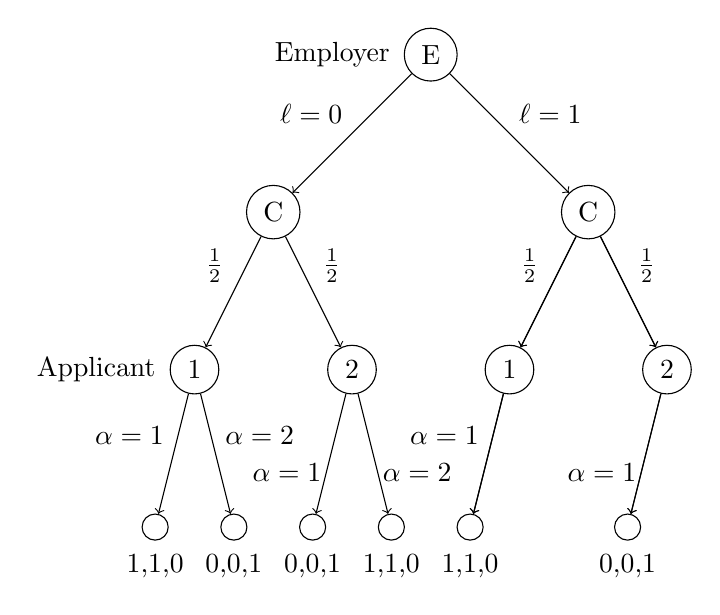
\begin{tikzpicture}
  \node[circle,draw] (1) at (0,0) {E}; % Chance Node
  \node[circle,draw] (2) at (-2,-2) {C}; % k=1 is strategic
  \node[circle,draw] (3) at (2,-2) {C}; % k=2 is strategic
  \node[circle,draw] (4) at (-3,-4) {1};
  \node[circle,draw] (5) at (-1,-4) {2};
  \node[circle,draw] (6) at (-3.5,-6) {};
  \node[circle,draw] (8) at (-2.5,-6) {};
  \node[circle,draw] (9) at (-1.5,-6) {};
  \node[circle,draw] (11) at (-0.5,-6) {};
  \node[circle,draw] (12) at (1,-4) {1};
  \node[circle,draw] (13) at (3,-4) {2};
  \node[circle,draw] (15) at (2.5,-6) {};
  \node[circle,draw] (17) at (0.5,-6) {};

  \node at (-1.25,0) {Employer};
  \node at (-4.25,-4) {Applicant};
  \node at (-3.5,-6.5) {1,1,0};
  \node at (-2.5,-6.5) {0,0,1};
  \node at (-1.5,-6.5) {0,0,1};
  \node at (-0.5,-6.5) {1,1,0};
  \node at (0.5,-6.5) {1,1,0};
  \node at (2.5,-6.5) {0,0,1};
  
  \draw[->] (1) to node[above left]{$\ell = 0$} (2);
  \draw[->] (1) to node[above right]{$\ell = 1$} (3);
  \draw[->] (2) to node[above left]{$\frac{1}{2}$} (4);   
  \draw[->] (2) to node[above right]{$\frac{1}{2}$} (5); 
  \draw[->] (3) to node[above left]{$\frac{1}{2}$} (12);   
  \draw[->] (3) to node[above right]{$\frac{1}{2}$} (13);  
  \draw[->] (4) to node[above left]{$\alpha = 1$} (6);  
  \draw[->] (4) to node[above right]{$\alpha = 2$} (8); 
  \draw[->] (5) to node[below left]{$\alpha = 1$} (9);  
  \draw[->] (5) to node[below right]{$\alpha = 2$} (11); 
  \draw[->] (12) to node[above left]{$\alpha = 1$} (17);  
  \draw[->] (13) to node[below left]{$\alpha = 1$} (15);  

  % Additional lines and arrows
  \draw[->] (3) to (12); % Arrow from node 2 to node 12 (G)
  \draw[->] (3) to (13); % Arrow from node 2 to node 13 (H)
  \draw[->] (12) to (17); % Arrow from node 12 (G) to node 6 (C)
  \draw[->] (13) to (15); % Arrow from node 13 (H) to node 15 (J)
  
\end{tikzpicture}}
\end{figure}

In the game tree above, the employer first selects $\ell$. Subsequently, nature determines the strategic candidate, with all candidates having an equal likelihood of being chosen. The chosen strategic candidate then selects an $\alpha$ to position themselves within the interview process. To find a robust $\ell$, the employer can simply sum the payoffs accrued in each branch of $\ell$ and select the one yielding the largest sum.
\\[2ex]
We call this $\ell^*$ and define it as follows
$$ \ell^* = \argmax_{\ell} \sum_{k=1}^{n}u_e(\ell,k)$$
$$ \iff \ell^* = \argmax_{\ell} \sum_{k=1}^{n}
\begin{cases}
    1 & \text{ if } k = 1 \\
    0 & \text{ if } k \neq 1 \text{ and } \ell = 0 \\
    \frac{\ell!(n-\ell-1)!}{(n-1)!}\sum_{i = 2}^{k-1}\binom{n-(i+1)}{\ell-1}\frac{1}{i-1} & \text{ if } \ell < \frac{(n-\ell-1)!(n-k)!}{(n-2)!(n-k-\ell)!} \\
    \frac{\ell}{n-1}\sum_{i = \ell + 1}^{n-1}\frac{1}{i-1} & \text{ if } \ell \geq \frac{(n-\ell-1)!(n-k)!}{(n-2)!(n-k-\ell)!}
\end{cases}
$$

We choose the $\ell$ that has the highest sum of probabilities of choosing the best candidate across all potential strategic candidates $k$. As the employers utility function is a complex piece wise function involving factorials, binomial coefficients and summations, it is too complex to find the argmax analytically so we solved it numerically. The employer's utility function involves factorials, binomial coefficients, and summations, which makes it non-linear and non-convex. These characteristics make it difficult to find the maximum of the function analytically, as standard optimization techniques like taking the derivative and setting it equal to zero do not apply. We first define the $\ell$ used in the classic secretary problem for $n$ candidates as $C^*$. A comparison between $\ell^*$ and $C^*$ can be seen later in Figure \ref{fig:SuccessRateComparison} and Table \ref{tab:Comparison}. 

\begin{lemma}\label{lemma:l*_upper_bound}
    $\ell^*$ is upper bounded by $\lfloor \frac{n-1}{2} \rceil$.
    \begin{proof}
        As shown in Lemma \ref{lemma:k=2_switching_point} the largest switching point is when $k=2$ is strategic. There is no reason to further increase $\ell$ after this and it would only lead to the employers utility decreasing as the probability of the best ranked candidate appearing in the first $\ell$ increases.
    \end{proof}
\end{lemma}

\begin{conjecture}\label{conjecture:l*_upper_bound}
    We conjecture that a lower bound for $\ell^*$ is $C^*$. \\
    The competitive secretary problem studied in this thesis is almost like the classic secretary problem from the employers perspective but there is an added ability to push the strategic applicant towards the end which would benefit the employer as then it is the same as the classic secretary problem but with one less candidate thus there is only ever a reason to choose an an $\ell \geq C^*$. 
\end{conjecture}

\subsection{Asymptotic Behaviour of Robust \texorpdfstring{$\ell$}{l}}

We now investigate the behaviour of $\ell^*$ as $n$ grows to infinity. Due to the complex expression of $l^*$, we were only able to perform numerical experiments to observe the asymptotic behaviour of $\ell^*$. After running multiple numerical experiments for increasingly larger values of $n$, we believe $\ell^*$ converges to $\frac{n}{e}$ but at a much slower rate than the classic secretary problem. This also leads to the employers utility converging to $e^{-1}$ as $n$ tends towards infinity. This is because as $n$ tends towards infinity the probability of any candidate $k$ being strategic converges to 0. Thus, as seen in Figure \ref{fig:switching_points} only the top 3 ranked candidates want to choose $\alpha=1$ when $\ell=\frac{n}{e}$ is chosen, hence, in the limit there is probability 0 that one of these candidates is the strategic candidate meaning we end up in the final case of the employers utility function defined in Theorem \ref{theorem:employer_utlity_best_response}. This function which is the same as classic secretary problem with one less applicant converges to $e^{-1}$ in the limit as having one less candidate does not make a difference when there are an infinite number of candidates. The limit of the summation in this case converges to 1 with $\ell=\frac{n}{e}$. The fraction before it converges to $e^{-1}$.

\begin{figure}[H]
\centering
\centering
\includegraphics[width=0.7\textwidth, keepaspectratio]{LongRunRelationship.png}
\caption{Long Run Relationship Between $\ell^*$, employer utility and $n$}
\label{fig:N-grows}
\end{figure}

% \begin{figure}[H]
% \centering
% \centering
% \includegraphics[width=\linewidth]{LongRun.png}
% \caption{Relationship}
% \label{fig:N-grows}
% \end{figure}

% \begin{itemize}
%     \item Explain Why $\ell^*$ Converges to $\frac{n}{e}$: You state that you believe $\ell^*$ converges to $\frac{n}{e}$, but you don't explain why. Providing some intuition or reasoning for this would strengthen your argument. For example, you could discuss how the strategic behavior of the candidates affects the optimal value of $\ell$.
%     \item Discuss the Implications of Your Results: How does the behavior of $\ell^*$ affect the employer's strategy? What does it mean for the employer's utility to converge to $e^{-1}$? Discussing the implications of your results can help readers understand their significance.
%     \item Address Potential Limitations: Are there any limitations or potential sources of error in your numerical experiments? How might these affect your results? Addressing potential limitations can help readers assess the reliability of your findings.
%     \item Future Work: Based on your findings, what are some potential directions for future research? For example, you might suggest analytical methods to confirm the asymptotic behavior of $\ell^*$, or you might propose studying the behavior of $\ell^*$ in different variants of the secretary problem.
% \end{itemize}


\section{Non Uniform Probabilities of Being Strategic Candidate}

Until now we have been assuming that the probability that a specific candidate $k$, is strategic is uniform across all $k$. That is we have given them equal weights, $w_k = \frac{1}{n}$. In this section we relax this assumption and explore what happens if we use different weighting systems to weight the likelihood of candidate $k$ being strategic. We choose decreasing weighting systems as we thought this would yield more interesting results and a decreasing weighting system because we wanted to model a situation where higher-ranked candidates are more likely to be strategic, reflecting the fact that these candidates often have more options and therefore more opportunity to be strategic in their behavior. A uniform weighting system was used initially as this is what is used in the classical secretary problem and is a natural first choice.

\subsection{Linear Decreasing Weight}

A linear decreasing weighting system is used here and the weights are given by 
$$ w_k = \frac{\frac{2}{n}(n-(k-1))}{n(n+1)} $$

% \begin{figure}[H]
% \centering
% \centering
% \includegraphics[width=\linewidth]{LinearDecreasingFixed.png}
% \caption{Linear Decreasing Probability Secretary Problem}
% \label{fig:linear_decreasing}
% \end{figure}

\begin{table}[H]
\centering
\begin{minipage}{0.5\textwidth}
\small
\begin{figure}[H]
\centering
\centering
\includegraphics[width=\linewidth]{LinearDecreasingFixed.png}
\caption{Linear Decreasing Probability Secretary Problem}
\label{fig:linear_decreasing}
\end{figure}
\end{minipage}\hfill
\centering
\begin{minipage}{0.49\textwidth}
\small
\begin{figure}[H]
\centering
\centering
\includegraphics[width=\linewidth]{EmployerUtilityLinearDecreasing.png}
\caption{Linear Decreasing Probability Secretary Problem}
\label{fig:linear_decreasing_employer_utility}
\end{figure}
\end{minipage}\hfill
\end{table}

The first plot on the left is similar to that presented above in figure \ref{fig:N-grows}. We can see that eventually for large enough $n$ the search fraction and probability of picking the best converge to roughly the same number and towards $e^{-1}$. The second plot on the left is very similar to that when using uniform weights as can be seen in figure \ref{fig:Employer_utility_uniform} but all the utilities are increased for each different $\ell$. The second peak is what explains the sudden drop in the first image, as the probabilities are favoured towards the better ranked candidates a higher search fraction is optimal as it will push more of the candidates towards the back and the probability of the best ranked candidate being in the first $\ell$ is lower as there higher probability that candidate is be strategic but at some point there is simply too many candidates which reduce the probability of the strategic candidate being $k=1$. Compared to the uniform weighting system, the linear decreasing weighting system results in a higher optimal search fraction and higher employer utility. This suggests that when higher-ranked candidates are more likely to be strategic, the employer can benefit from conducting a more extensive search.

\subsection{Exponential Decreasing Weight}

An exponential decreasing weighting system is applied here. An exponential decreasing weight system is a method of assigning weights that decrease exponentially. This means that each subsequent weight is a fixed proportion less than the previous weight. This type of weighting system is often used in situations where the importance or relevance of an item (in this case, a candidate) decreases rapidly. We chose an exponential decreasing weighting system to model a situation where the likelihood of a candidate being strategic decreases rapidly as their rank decreases. This could reflect a situation where only the top few candidates have the resources or inclination to be strategic. The weights are given by 
$$ w_k = \frac{\frac{1}{n}2^{n-(k-1)}}{2^{n+1}-1} $$
In the formula $w_k = \frac{\frac{1}{n}2^{n-(k-1)}}{2^{n+1}-1}$, $w_k$ represents the weight of the $k$th candidate, $n$ is the total number of candidates, and $k$ is the rank of a candidate. The numerator $\frac{1}{n}2^{n-(k-1)}$ represents the unnormalised weight of the $k$th candidate, and the denominator $2^{n+1}-1$ is a normalization factor that ensures that the sum of all weights equals 1.

% \begin{figure}[H]
% \centering
% \centering
% \includegraphics[width=\linewidth]{ExponentialDecreasingFixed.png}
% \caption{Exponential Decreasing Probability Secretary Problem}
% \label{fig:exponential_decreasing}
% \end{figure}

\begin{table}[H]
\centering
\begin{minipage}{0.5\textwidth}
\small
\begin{figure}[H]
\centering
\centering
\includegraphics[width=\linewidth]{ExponentialDecreasingFixed.png}
\caption{Exponential Decreasing Probability Secretary Problem}
\label{fig:exponential_decreasing}
\end{figure}
\end{minipage}\hfill
\centering
\begin{minipage}{0.5\textwidth}
\small
\begin{figure}[H]
\centering
\centering
\includegraphics[width=\linewidth]{EmployerUtilityExponentialDecreasing.png}
\caption{Exponential Decreasing Probability Secretary Problem}
\label{fig:exponential_decreasing_employer_utility}
\end{figure}
\end{minipage}\hfill
\end{table}

We can see that when an exponential weighting system is used the search fraction and employers utility never converge to the same value. We also observe that there are jumps in the utility for different values of $\ell$, particularly when $\ell=\lfloor \frac{n-1}{2} \rceil$ is chosen. This is due to the extreme weighting in favour of higher ranked candidates.


\subsection{Harmonic Decreasing Weight}

A harmonic decreasing weighting system is used here. We chose a harmonic decreasing weighting system to model a situation where the likelihood of a candidate being strategic decreases at a slower rate as their rank decreases. This could reflect a situation where even lower-ranked candidates have a significant chance of being strategic. The weights are given by 
$$ w'_k = \frac{\frac{\frac{1}{n}}{\sum_{i=1}^{n}\frac{1}{i+1}}}{k}$$
and 
$$ w_k = \frac{w'_k}{\sum_{i=1}^{n}w'_k}$$

% \begin{figure}[H]
% \centering
% \centering
% \includegraphics[width=\linewidth]{HarmonicDecreasingFixed.png}
% \caption{Harmonic Decreasing Probability Secretary Problem}
% \label{fig:harmonic_decreasing}
% \end{figure}

\begin{table}[H]
\centering
\begin{minipage}{0.5\textwidth}
\small
\begin{figure}[H]
\centering
\centering
\includegraphics[width=\linewidth]{HarmonicDecreasingFixed.png}
\caption{Harmonic Decreasing Probability Secretary Problem}
\label{fig:harmonic_decreasing}
\end{figure}
\end{minipage}\hfill
\centering
\begin{minipage}{0.5\textwidth}
\small
\begin{figure}[H]
\centering
\centering
\includegraphics[width=\linewidth]{EmployerUtilityHarmonicDecreasing.png}
\caption{Harmonic Decreasing Probability Secretary Problem}
\label{fig:harmonic_decreasing_employer_utility}
\end{figure}
\end{minipage}\hfill
\end{table}

The results show that the optimal search fraction and employer utility converge towards the same value but at a higher level than in the uniform weighting case. This suggests that when the likelihood of a candidate being strategic decreases slowly with their rank, the employer can benefit from conducting a more extensive search. For a fixed $n$ we see that the employers utility is maximised when an $\ell=\lfloor \frac{n-1}{2} \rceil$ is chosen. The weighing is not as extreme as in the previous case and would explain why the utility of choosing this $\ell$ is not as high. 

\section{Comparison of Classic to Competitive}

In the classic secretary problem the utility the employer receives for choosing different $\ell$ is the probability of selecting the best candidate and is given by 
$$ u_e(\ell) =
\begin{cases}
    \frac{1}{n} & \text{ if } \ell = 0 \\
    \frac{\ell}{n} \sum_{i=\ell+1}^{n}\frac{1}{i-1} & \text{ if } \ell \neq 0
\end{cases}$$

The following figure displays the search fraction and employers utility for different total number of candidates $n$.


\begin{figure}[H]
\centering
\centering
\includegraphics[width=0.7\textwidth, keepaspectratio]{Classic Secretary Problem.png}
\caption{Classic Secretary Problem}
\label{fig:Classic_Secretary_Problem}
\end{figure}

The following tables and graph will compare the classic and competitive secretary problems, both $\ell^*$ and $C^*$ are presented as fractions of $n$.

\begin{table}[H] 
\centering
\begin{minipage}{0.5\textwidth}
\small
\begin{tabular}{lrr} 
\hline
$n$ & $\frac{C^*}{n}$ & Employer utility \\
\hline
1  &     0 &         1 \\
2  &     0 &         0.5 \\
3  &     0.3333 &         0.5 \\
4  &     0.25 &         0.4583 \\
5  &     0.4 &         0.4333 \\
6  &     0.3333 &         0.4278 \\
7  &     0.2857 &         0.4143 \\
8  &     0.375 &         0.4098 \\
9  &     0.3333 &         0.4060 \\
10 &     0.3 &         0.3987 \\
\hline
\end{tabular}
\caption{$C^*$ and corresponding employer utility}
\label{tab:Comparison}
\end{minipage}\hfill
\centering
\begin{minipage}{0.5\textwidth}
\small
\begin{tabular}{lrr}
\hline
$n$ & $\frac{\ell^*}{n}$ & Employer utility \\
\hline
1  &     0 &         1 \\
2  &     0 &         0.5 \\
3  &     0.3333 &         0.6667 \\
4  &     0.25 &         0.5 \\
5  &     0.4 &         0.5333 \\
6  &     0.5 &         0.4583 \\
7  &     0.4286 &         0.4786 \\
8  &     0.5 &         0.4333 \\
9  &     0.4444 &         0.4487 \\
10 &     0.5 &         0.4173 \\
\hline
\end{tabular}
\caption{$\ell^*$ and corresponding employer utility}
\end{minipage}\hfill
\end{table}


\begin{table}[H]
\centering
\begin{minipage}{0.5\textwidth}
\small
\begin{figure}[H]
\centering
\centering
\includegraphics[width=\linewidth]{SuccessRateComparison.png}
\caption{Success Rate Comparison}
\label{fig:SuccessRateComparison}
\end{figure}
\end{minipage}\hfill
\centering
\begin{minipage}{0.49\textwidth}
\small
\begin{figure}[H]
\centering
\centering
\includegraphics[width=\linewidth]{SearchFractionComparison.png}
\caption{Search Fraction Comparison}
\label{fig:SearchFractionComparison}
\end{figure}
\end{minipage}\hfill
\end{table}

In the above graph it can be seen that the success rate of the employer is always at least as large as the success rate in the classic setting and the majority of the time it is higher. Additionally, the search rate is always at least as large as it is in the classic setting and the majority of the time it is slightly higher, this is because as $\ell$ increases more candidates will switch to the final position which is advantageous for the employer as it is essentially the classic secretary problem but with one less candidate.

\subsection{Competition Improving Utilities}

The first striking observation from this introduced competitive setting is that competition improves each players expected utility, both employer and strategic candidate have a higher probability of achieving the outcome they would like compared to the classic secretary problem.

\subsubsection{Employer}

The employer in the classic secretary problem has a probability of $e^{-1}$ of selecting the best candidate in the limit and for smaller $n$ the employers utility can be seen in Table \ref{tab:Comparison} and Figure \ref{fig:SuccessRateComparison}. As can be seen the employer almost always has a greater utility in the competitive setting and when $n$ tends towards infinity the utility is the same but it converges at a much slower rate. Hence, in most situations the employer is better off that there is a strategic candidate with a choice.

\subsubsection{Candidate}

In the classic secretary problem candidates have a probability upper bounded by $e^{-1}$, as this is the probability of selecting the best ranked candidate it must certainly be smaller for lower ranked candidates. In this competitive setting candidates have probabilities presented in Theorem \ref{theorem:applicant_probabilities}. In this case where the candidate is sufficiently low ranked that they have a probability of 0 of being selected if they choose $\alpha=1$ they will choose $\alpha=(n-\ell)$ which leads to a probability of $\frac{\ell}{n-1}$ of being selected which is greater than 0 for all $\ell \in \{ 1, \ldots, (n-1) \} $. For the second ranked candidate it was shown that they also benefit from this added competition. Of course the added competition involves giving the applicant a choice as to where to position themselves which should certainly improve their utility, it can not make it worse. The fact that the employer also benefits is what is remarkable.

\section{Applicant Unaware of their Rank}

A candidate with no knowledge of their rank will assume there is a $\frac{1}{n}$ chance that they are of rank $k$ in the original formulation of the problem. To find their best strategy in response to $\ell$ they would choose the 
$$ \alpha^* = \argmax_{\alpha} \sum_{k=1}^{n} u_k(\ell, \alpha) $$
That is the $\alpha$ which would maximise their probability of being picked. To calculate $\alpha^*$ we use the $\ell^*$ calculated earlier and plug it into the utility function defined in Theorem \ref{theorem:applicant_probabilities}.
\\[2ex]
As we saw earlier a $\ell=\frac{n}{e}$ leads to almost all the candidates choosing to position themselves at the end, which would also be robust $\alpha$ choice, if you had no information regarding your rank. This means in the limit the second payoff is what is important. We can see that for the second payoff plugging in this $\ell$, in the limit will lead to a probability of being selected of $\frac{1}{e}$ for the candidate who is unaware of their rank and chooses an $\alpha=(n-\ell)$.

\section{Multiple Strategic Candidates}

If the game were to be defined differently and allow for multiple strategic candidates it would require priority be given to one of the players should they choose the same $\alpha$. We will briefly explore what would change in the game should there be multiple strategic candidates. First we will fix it to two strategic candidates. These candidates have rank $k$ and $k'$. First, we will give candidate $k$ first choice meaning $k'$ is in a more advantageous position, it can be represented with the following game tree


\begin{figure}[H]
\centering
\scalebox{1}{
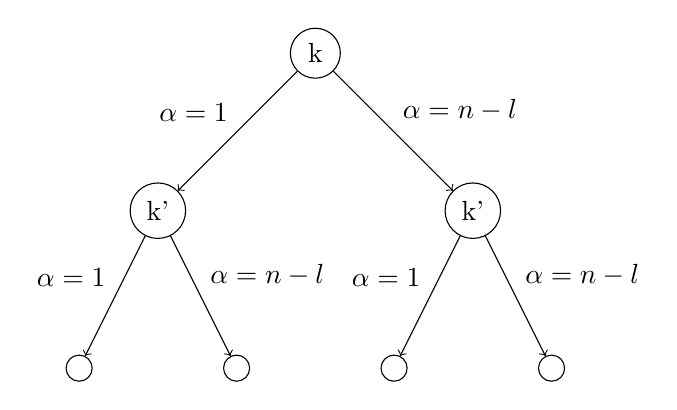
\begin{tikzpicture}
  \node[circle,draw] (1) at (0,0) {k}; % Chance Node
  \node[circle,draw] (2) at (-2,-2) {k'}; % k=1 is strategic
  \node[circle,draw] (3) at (2,-2) {k'}; % k=2 is strategic
  \node[circle,draw] (4) at (-3,-4) {};
  \node[circle,draw] (5) at (-1,-4) {};
  % \node[circle,draw] (6) at (-3.5,-6) {};
  % \node[circle,draw] (8) at (-2.5,-6) {};
  % \node[circle,draw] (9) at (-1.5,-6) {};
  % \node[circle,draw] (11) at (-0.5,-6) {};
  \node[circle,draw] (12) at (1,-4) {};
  \node[circle,draw] (13) at (3,-4) {};
  % \node[circle,draw] (14) at (3.5,-6) {I};
  % \node[circle,draw] (15) at (2.5,-6) {};
  % \node[circle,draw] (16) at (1.5,-6) {K};
  % \node[circle,draw] (17) at (0.5,-6) {};

  % \node at (-1.25,0) {Employer};
  % \node at (-4.25,-4) {Applicant};
  % \node at (-3.5,-6.5) {1,1,0};
  % \node at (-2.5,-6.5) {0,0,1};
  % \node at (-1.5,-6.5) {0,0,1};
  % \node at (-0.5,-6.5) {1,1,0};
  % \node at (0.5,-6.5) {1,1,0};
  % \node at (1.5,-6.5) {0,0,1};
  % \node at (2.5,-6.5) {0,0,1};
  % \node at (3.5,-6.5) {1,0};
  
  % \draw[dashed] (2) to node[above] {} (3);
  \draw[->] (1) to node[above left]{$\alpha=1$} (2);
  \draw[->] (1) to node[above right]{$\alpha = n-l$} (3);
  \draw[->] (2) to node[above left]{$\alpha=1$} (4);   
  \draw[->] (2) to node[above right]{$\alpha = n-l$} (5); 
  \draw[->] (3) to node[above left]{$\alpha=1$} (12);   
  \draw[->] (3) to node[above right]{$\alpha = n-l$} (13);  
  % \draw[->] (4) to node[above left]{$\alpha = 1$} (6);  
  % \draw[->] (4) to node[above right]{$\alpha = 2$} (8); 
  % \draw[->] (5) to node[below left]{$\alpha = 1$} (9);  
  % \draw[->] (5) to node[below right]{$\alpha = 2$} (11); 
  % \draw[->] (12) to node[above left]{$\alpha = 1$} (17);  
  % \draw[->] (12) to node[above right]{$\alpha = 2$} (16); 
  % \draw[->] (13) to node[below left]{$\alpha = 1$} (15);  
  % \draw[->] (13) to node[below right]{$\alpha = 2$} (14); 

  % Additional lines and arrows
  % \draw[->] (3) to (12); % Arrow from node 2 to node 12 (G)
  % \draw[->] (3) to (13); % Arrow from node 2 to node 13 (H)
  % \draw[->] (12) to (17); % Arrow from node 12 (G) to node 6 (C)
  % \draw[->] (12) to (16); % Arrow from node
  % \draw[->] (12) to (16); % Arrow from node 12 (G) to node 16 (K)
  % \draw[->] (13) to (15); % Arrow from node 13 (H) to node 15 (J)
  % \draw[->] (13) to (14); % Arrow from node 13 (H) to node 14 (I)
  
\end{tikzpicture}}
\end{figure}

This game tree would be added onto the game tree that includes the employers decision. This then is the subgame concerning the two strategic applicants. 
\\[2ex]
The choice of $k'$ in each subgame is similar to that in the normal game but there is the added information of where $k$ will position themselves. If $k=1$ then $k'$ must choose $\alpha=1$ as any other choice will lead to $k$ being selected.
\\[2ex]
If $k>k'$ the payoff for $k'$ for choosing $\alpha=1$ is 
$$\frac{\ell!(n-\ell-2)!}{(n-2)!}\binom{n-k'-1}{\ell}$$
Using the result obtained in Theorem \ref{theorem:applicant_probabilities}, since $k$ has already made their choice there is now only $(n-\ell-2)$ people to permute after $k$ and $k'$ have made their choice. The denominator also becomes $(n-2)$ as everyone needs to be permuted apart from the two making a choice. In the binomial there is one less person that can be chosen in the first $\ell$ that will insure that $k'$ can still be selected as $k$ has a higher rank than $k'$. The payoff for $k'$ for choosing $\alpha=(n-\ell)$ is 
$$\frac{\ell}{n-2}$$
as there is now one extra person that will not appear in the first $l$ which increases the chances that $k=1$ appears in the first $\ell$.
\\[2ex]
If $k<k'$, the payoff for choosing $\alpha=(n-\ell)$ is as above $$\frac{\ell}{n-2}$$
as there are two people who are fixing their position and will not appear in the first $\ell$. The payoff for choosing $\alpha=1$ is obtained as above from Theorem \ref{theorem:applicant_probabilities} and above
$$\frac{\ell!(n-\ell-2)!}{(n-2)!}\binom{n-k'}{\ell}$$
The number of of people to permute has decreased and the number of other applicants worse than $k'$ remains the same.
\\[2ex]
Going up the game tree we now consider the choice of $k$. If $k'$ is choosing $\alpha=(n-l)$ then $k$ can not choose $\alpha=(n-l)$, as it would be inferior to $\alpha=1$ as shown in Lemma \ref{lemma:dominated}, since $k$ would actually be positioned at $\alpha=(n-l-1)$. If $k'$ chooses $\alpha=1$ the payoff for $k$ for choosing $\alpha=(n-l)$ is $\frac{\ell}{n-2}$. The payoff for choosing $\alpha=1$ depends on whether $k'$ is better or worse ranked than $k$. If $k>k'$ the payoff would be zero as there will be someone better before you and they will always be picked. The payoff if $k<k'$ will be similar to that defined before but $k$ is picked if someone better than $k'$ but worse than $k$ appears in $\ell$.


% \subsection{Generalising to multiple strategic candidates}

% The payoff for choosing $\alpha=(n-\ell)$ becomes 
% $$\frac{\ell}{n-s} $$
% where $s = |S|$ and $S$ is the set of strategic candidates. The payoff for choosing $\alpha=1$ depends on the number of strategic candidates that are better or worse than you. Thus there would now be $(n-(k'-b)-w)$ who can be chosen in the first $\ell$. Where $b$ refers to the number of strategic candidates that are better ranked than you and $w$ refers to the number of strategic candidates that are worse ranked than you. Thus the payoff for choosing $\alpha=1$ is 
% $$\frac{\ell!(n-\ell-s)!}{(n-s)!}\binom{n-(k'-b)-w}{\ell}$$

\section{Future Research}

In the following section, we discuss some potential avenues for future research. Extensions to the model or other areas of research related to this model.

\subsection{Unknown Total Number of Candidates}

An extension to this model could involve reducing the employers information regarding how many applicants there are and only providing the employer with an upper bound. This extension to the classic secretary problem was studied by \cite{freeman1983secretary}. This extension is fitting as in many cases the employer will not know the total number of applicants to a position when the first interview begins and likewise for the framing of "The Marriage Problem", you will not know how many people you date in life and so as the decision maker taking this uncertainty into account may lead to a more optimal strategy for real life applications of this secretary problem. Regarding the competitive variant studied in this thesis, there could be two versions studied, one where the strategic applicant is made aware of the total number of candidates and another where they are not. In the variant where they are not, the strategy space of the strategic applicant would need to be redefined and possibly incorporate some kind of belief as to what the total number of applicants is. Additionally, it would now become harder for the employer to define an $\ell$ as a fraction of $n$ as $n$ is now unknown and so would also require the employer to have some prior belief regarding the total number of interviews to take place. In this scenario where the total number of candidates is unknown, the strategic applicant's decision-making process could be influenced by a variety of factors. For instance, they might base their decisions on their perceived competitiveness in the applicant pool, their urgency to secure a position, or their assumptions about the employer's hiring strategy. Bayesian decision theory could be a useful framework for modeling the applicant's beliefs and decision-making process in this context. On the other hand, the employer might need to adjust their hiring strategy to account for the uncertainty about the total number of candidates. They might choose to be more conservative, hiring a strong candidate early on to avoid the risk of not finding a better candidate later. Alternatively, they might choose to be more aggressive, waiting for a truly outstanding candidate and risking the possibility that such a candidate might not appear. The optimal strategy could depend on factors such as the employer's risk tolerance and the cost of not filling the position.

\subsection{Multiple Competing Employers}

Instead of having just a single employer, there could be multiple competing employers all vying for the best candidate or they could simply be trying to beat the hires of the other employers as was studied by \cite{immorlica2011dueling}. Adding this extension to this competitive variant with ranked employers (to break ties) would be very interesting. The strategic candidate would need to decide whether they prioritise getting hired or getting hired by the best ranking employer as this would change which $\alpha$ they prefer. This would also be highly dependent on their rank. The strategic applicant, for instance, would need to weigh the benefits of securing a position against the potential benefits of holding out for an offer from a higher-ranking employer. Game theory, particularly the concept of Nash equilibrium, could provide valuable insights into the decision-making processes in this scenario. The presence of multiple employers could also create a more competitive environment, as each employer would be vying to secure the best candidates. This could lead to a 'race' among employers, with each trying to make attractive offers before their competitors do. Alternatively, employers might choose to cooperate, sharing information and coordinating their hiring decisions to avoid unnecessary competition. The optimal strategy for each employer could depend on factors such as the number of competitors, the quality of the applicant pool, and the cost of not filling a position.

\subsection{Empirical Research}

To empirically test the model, an experimental study could be designed where participants are randomly assigned to the roles of employer or strategic applicant. Participants could be recruited from a variety of sources, such as online platforms, universities, or professional networks, to ensure a diverse sample. In the experiment, participants would be presented with a series of decision-making tasks, representing different stages of the hiring process. They would be provided with varying levels of information about the other participants and the overall state of the game, and their decisions and outcomes would be recorded for analysis. Some potential challenges in conducting such an experiment could include ensuring that participants understand the rules of the game, maintaining their engagement throughout the experiment, and dealing with potential biases in their decision-making. These challenges could be addressed through careful experimental design, such as providing clear instructions and feedback, incorporating elements of gamification to maintain engagement, and using statistical methods to control for potential biases in the analysis.

\section{Conclusion}

This thesis has presented a novel extension to the classic secretary problem by introducing a competitive element where one of the candidates can strategically position themselves in the interview process. We have explored the optimal strategies for both the employer and the strategic candidate under different conditions and assumptions.
\\[2ex]
We found that the introduction of competition generally improves the expected utilities for both the employer and the strategic candidate. The employer benefits from the strategic candidate's tendency to position themselves later in the interview process, effectively reducing the pool of candidates and increasing the probability of selecting the best candidate. The strategic candidate, on the other hand, can increase their chances of being selected by choosing an optimal position in the interview process. We study the asymptotic strategies of both players as the number of applicants tends towards infinity and the players choices when restricting their information.
\\[2ex]
We also investigated the impact of different weighting systems on the likelihood of a candidate being strategic. We found that the optimal strategies and utilities can vary significantly depending on the weighting system used, highlighting the importance of understanding the underlying distribution of strategic behavior among candidates. This thesis can also contribute to growing study of the relationship between secretary problems and online auctions, as studied by \cite{hajiaghayi2004adaptive} and \cite{babaioff2008online}.
\\[2ex]
In terms of future work, it would be interesting to explore other types of strategic behavior, such as candidates being able to influence their ranking or the employer's perception of their ranking. Additionally, it would be worthwhile to investigate the impact of multiple strategic candidates or multiple employers and the potential for strategic interactions between them. Future work could also involve conducting an empirical experiment. 

\newpage

\bibliography{ref.bib}

\newpage

\begin{appendices}
\section{SDG Statement}
The competitive secretary problem is closely linked to the United Nations' sustainable development goal of "Decent Work and Economic Growth" (SDG 8) \citeyear{unitednations}. The problem of selecting the best candidate out of a pool of applicants, is a problem facing every firm almost all the time. By selecting the best candidate, companies can improve their productivity and overall performance, which in turn leads to economic growth. Additionally, by selecting the best candidate, companies can also provide decent work opportunities for individuals, which is a key aspect of SDG 8. Furthermore, the competitive secretary problem highlights the importance of effective decision-making and fair recruitment practices, both of which are crucial for achieving SDG 8. The fairness of the recruitment process is achieved by the fact that the algorithms are designed so as not to discriminate between applicants. This thesis will also help potential employees as it will give insights regarding optimal strategies for approaching the hiring process.
\includepdf[pages={1-}]{SDG_Statement}	

\newpage

% \section{Additional Weighting Systems}

% \subsection{Geometric Decreasing Weight}

% \textbf{Put this in Appendix}

% A geometric decreasing weighting system with parameter $r = 0.8$ is used here and the weights are given by 
% $$ w_k(r) = \frac{1}{n}\frac{1-r}{1-r^{n}}r^{k-1} $$
% where $r$ is ratio to determine the rate at which the weights change.

% \begin{figure}[H]
% \centering
% \centering
% \includegraphics[width=\linewidth]{GeometricDecreasingFiex.8.png}
% \caption{Geometric Decreasing Probability Secretary Problem}
% \label{fig:geo_d}
% \end{figure}

% \subsection{Decaying Decreasing Weight}

% \textbf{Put this in Appendix}

% A decaying decreasing weighting system is used here and the weights are given by 
% $$ w'_k(r) = e^{-r(k-1)}$$ 
% and 
% $$ w_k(r) = \frac{w'_k(r)}{\sum_{k=1}^{n} w'_k(r)}$$ 


% \begin{figure}[H]
% \centering
% \centering
% \includegraphics[width=\linewidth]{DecayingDecreasingFixed.5.png}
% \caption{Decaying Decreasing Probability Secretary Problem}
% \label{fig:N-grows}
% \end{figure}

\end{appendices}

\end{document}
